\chapterimage{orange2.jpg}
\chapterspaceabove{6.75cm} 
\chapterspacebelow{7.25cm} 
\chapter{Set, Sequence, Function, and Summation}
\section{Set}
    We begin our formal development with basic notions of set theory. Our most primitive notion is that of a set. This notion is so fundamental that we do not attempt to give a precise definition. We think of a set as a collection of distinct objects with a precise description that provides a way of deciding (in principle) whether a given object is in it.

\begin{definition}[Set]
The objects in a set are its elements or members. When \( x \) is an element of \( A \), we write \( x \in A \) and say ``\( x \) belongs to \( A \)". When \( x \) is not in \( A \), we write \( x \notin A \). If every element of \( A \) belongs to \( B \), then \( A \) is a subset of \( B \), and \( B \) contains \( A \); we write \( A \subseteq B \) or \( B \supseteq A \).
\end{definition}

\begin{remark}
By convention, we use the special characters \( \mathbb{N} \), \( \mathbb{Z} \), \( \mathbb{Q} \), \( \mathbb{R} \) to name the sets of natural numbers, integers, rational numbers, and real numbers, respectively. Each set in this list is contained in the next, so we write \( \mathbb{N} \subseteq \mathbb{Z} \subseteq \mathbb{Q} \subseteq \mathbb{R} \).
\end{remark}

Sets Could be expressed in different ways. For sets with limited and few elements, we simply list all the elements in a pair of bracket, such as $A = \{1, 2, 3, 4, 5\}$. For sets with more elements, we can also define a set by description: $A = \{x: x\in \mathbb{Z^+} \text{ and } x \leq5 \}$. For example:
\begin{example}
    The rational number set could be expressed as:
    $$\mathbb{Q} = \{x: x\in \mathbb{R}, x = \frac{p}{q} \text{ where } p, q \in \mathbb{Z},\text{ but } q \neq 0\}$$
\end{example}

\begin{definition}[Equality of Sets]
Sets \( A \) and \( B \) are equal, written \( A = B \), if they have the same elements. The empty set, written \( \emptyset \), is the unique set with no elements. A proper subset of a set \( A \) is a subset of \( A \) that is not \( A \) itself. The power set of a set \( A \) is the set of all subsets of \( A \).
In other words, the complement of \( A \) includes everything that is not in \( A \).
\end{definition}



\begin{definition}[Basic Set operations]
Intersection, union and exclusion.
 \begin{itemize}
  \item the \textbf{intersection} of \( A \) and \( B \),
  \[ A \cap B = \{x : x \in A \text{ and } x \in B\}; \]
  \item the \textbf{union} of \( A \) and \( B \),
  \[ A \cup B = \{x : x \in A \text{ or } x \in B\}; \]
  \item the \textbf{set difference}, \( A \) but not \( B \),
  \[ A \setminus B = \{x : x \in A \text{ and } x \notin B\}. \]

\end{itemize}

The set \( A \setminus B \) is sometimes called the ``relative complement'' of \( B \) in \( A \).

When \( A \cap B = \emptyset \), sets \( A \) and \( B \) are said to be \textbf{disjoint}.
\end{definition}

\begin{definition}[Complement of Set]
The complement of a set \( A \), often denoted as \( \overline{A} \), $\sim A$ or \( A^c \), is defined with respect to a universal set \( U \), which contains all objects under consideration. The complement \( \overline{A} \) consists of all elements in \( U \) that are not in \( A \). Formally, if we have a universal set \( U \) and a subset \( A \subseteq U \), then the complement of \( A \) is given by:
\[ \overline{A} = \{ x \in U \mid x \notin A \} \]


\end{definition}
\begin{definition}[Intervals]
Intervals. When \( a, b \in \mathbb{R} \) with \( a < b \), the closed interval \( [a, b] \) is the set \( \{x \in \mathbb{R} : a \leq x \leq b\} \). The open interval \( (a, b) \) is the set \( \{x \in \mathbb{R} : a < x < b\} \).
\end{definition}


\section{Properties of Sets with Proofs}

\subsection*{Commutative Laws}
\textbf{Union:}
\[
A \cup B = B \cup A
\]
\textbf{Proof:} 
The union of sets \( A \) and \( B \) includes all elements that are in \( A \), in \( B \), or in both. Since the notion of "being in" does not depend on the order, \( A \cup B \) and \( B \cup A \) represent the same set.

\noindent\textbf{Intersection:}
$$A \cap B = B \cap A$$


\textbf{Proof:} 
The intersection of sets \( A \) and \( B \) includes all elements that are both in \( A \) and in \( B \). The order of \( A \) and \( B \) does not affect the elements that are shared between them, hence the equality.

\subsection*{Associative Laws}
\textbf{Union:}
\[
(A \cup B) \cup C = A \cup (B \cup C)
\]
\textbf{Proof:} 
When we take the union of sets, we combine their elements. Grouping does not affect the outcome of the union, thus the union operation is associative.

\textbf{Intersection:}
\[
(A \cap B) \cap C = A \cap (B \cap C)
\]
\textbf{Proof:} 
The intersection operation finds common elements. The grouping of sets does not affect the commonality of elements, so the intersection operation is associative.

\subsection*{Distributive Laws}
\textbf{Intersection distributes over union:}
\[
A \cap (B \cup C) = (A \cap B) \cup (A \cap C)
\]
\textbf{Proof:} 
An element in \( A \cap (B \cup C) \) is in \( A \) and either \( B \) or \( C \). This is the same as the element being in both \( A \) and \( B \), or in both \( A \) and \( C \).

\textbf{Union distributes over intersection:}
\[
A \cup (B \cap C) = (A \cup B) \cap (A \cup C)
\]
\textbf{Proof:} 
An element in \( A \cup (B \cap C) \) is in \( A \), in both \( B \) and \( C \), or in all. This is equivalent to the element being in \( A \) or \( B \), and in \( A \) or \( C \).

\subsection*{De Morgan's Laws}
\textbf{Complement of the union:}
\[
\overline{A \cup B} = \overline{A} \cap \overline{B}
\]
\textbf{Proof:} 
An element not in \( A \cup B \) is neither in \( A \) nor in \( B \), which means it is in both \( \overline{A} \) and \( \overline{B} \).

\textbf{Complement of the intersection:}
\[
\overline{A \cap B} = \overline{A} \cup \overline{B}
\]
\textbf{Proof:} 
An element not in \( A \cap B \) is not in both \( A \) and \( B \), which means it is either in \( \overline{A} \) or in \( \overline{B} \).

\subsection*{Properties of Complements}
\textbf{Union with complement:}
\[
A \cup \overline{A} = U
\]
\textbf{Proof:} 
The set \( A \) together with all elements not in \( A \) constitutes the entire universe \( U \).

\textbf{Intersection with complement:}
\[
A \cap \overline{A} = \emptyset
\]
\textbf{Proof:} 
No element can be both in set \( A \) and not in set \( A \) at the same time, hence the intersection is the empty set.

\begin{definition}[Subset]
    If $A$ and $B$ are sets, we say $A$ is a subset of $B$ if every element of $A$ is also an element of $B$. This is denoted as \(A \subseteq B\)  
\end{definition}
\begin{remark}
    Note that for every set, it is a subset to itself.
\end{remark}
\begin{definition}[Proper Subset]
    If \( B \subset A \), then \( B \) is a proper subset of \( A \).
\end{definition}
For instance, consider the set \( A = \{1, 2, 3\} \) and the set \( B = \{1, 2\} \). In this case, \( B \subset A \), because every element of \( B \) is in \( A \), but \( A \) contains an additional element \( 3 \) that is not in \( B \).
\begin{definition}[Empty Set]
    The \textbf{empty set} is a unique set that contains no elements. It is denoted as \( \varnothing \). This set is important in set theory because it serves as the identity element for the union operation and has properties that are fundamental to the construction of other sets. For example, every set, including the empty set itself, contains the empty set as a subset:

\[ \varnothing \subseteq A \]

for any set \( A \). Furthermore, the intersection of any set with the empty set is the empty set itself:

\[ A \cap \varnothing = \varnothing \]

This highlights the empty set's role in set operations.
\end{definition}

\begin{definition}[Power Set]
    If \( A \) is any set, the \textbf{power set} of \( A \),
\[ \mathcal{P}(A) = \{S: S \subseteq A \} \]
// the set of all subsets of \( A \)

For example, if \( A = \{a, b, c\} \) then
\[ \mathcal{P}(A) = \{\varnothing, \{a\}, \{b\}, \{c\}, \{a, b\}, \{a, c\}, \{b, c\}, \{a, b, c\} \}. \]
\end{definition}
\begin{definition}[cardinality]
    The number of elements in a set \( S \) is called the \textbf{cardinality} of \( S \) and denoted by \( |S| \). When this is a finite number, then \( |S| \in \mathbb{N} \), and when \( |S| = n \), we'll say that \( S \) is an \( n \)-set. 
\end{definition}
\begin{definition}[Partition of Sets]
    Each element of \( A \cup B \) is in exactly one of the sets \( A \setminus B \), \( B \setminus A \), and \( A \cap B \). More generally,

subsets \( S_1, S_2, S_3, \ldots, S_k \) of \( T \) form a \textbf{partition} of \( T \) means every element of \( T \) belongs to exactly one of the sets \( S_j \).
\end{definition}
The sets \( S_1 = A \setminus B \), \( S_2 = B \setminus A \) and \( S_3 = A \cap B \) form a partition of \( T = A \cup B \).
 In general, \( S_1 \cup S_2 \cup S_3 \ldots \cup S_k \subseteq T \) because each \( S_j \) is a subset of \( T \).
 \( T \subseteq S_1 \cup S_2 \cup S_3 \ldots \cup S_k \) because each element of \( T \) is in some subset \( S_j \).
 Therefore, \( T = S_1 \cup S_2 \cup S_3 \ldots \cup S_k \).

The subsets in a partition are \textbf{mutually disjoint}; that is, any two are disjoint sets.

 If \( p \neq q \), \( S_p \cap S_q = \emptyset \) because no element of \( T \) belongs to more than one \( S_j \).

When \( S_1, S_2, S_3, \ldots, S_k \) forms a partition of \( T \), then
\[ |T| = |S_1| + |S_2| + |S_3| + \ldots + |S_k|. \]


\begin{theorem}[The Principle of Inclusion-Exclusion]
    For any pair of sets,\[ |A \cup B| = |A| + |B| - |A \cap B|, \]

and when \( A \) and \( B \) are disjoint,

\[ |A \cup B| = |A| + |B|. \quad \text{// since } A \cap B = \emptyset \]

Furthermore, we always have

\[ |A \cup B| = |A \setminus B| + |B \setminus A| + |A \cap B|. \]
\end{theorem}

\begin{definition}[The Cartesian Product]
    \textbf{The Cartesian product} of sets \( A \) and \( B \), named for Ren\'e Descartes (1596--1650), is

\[ A \times B = \{(a, b): a \in A \text{ and } b \in B\}, \]

where \( (a,b) \) denotes an ordered pair of objects; there is a first entry and a second entry in each ordered pair. \emph{Parentheses} indicate that order matters.

% Braces indicate it doesn't.
\end{definition}
\begin{remark}
    \[ \{0, 1\} = \{1, 0\}, \text{ but } (0, 1) \neq (1, 0). \quad \text{-- in sets, order doesn't matter; in ordered pairs it does.} \]
    
\[ \{1, 1\} = \{1\}, \text{ but } (1, 1) \neq (1). \quad \text{-- in sets, repetitions don't matter; in ordered pairs they do.} \]

\end{remark}
\begin{example}
    If \( A = \{1,3,5,7\} \) and \( B = \{2,3,5\} \), then

\[ A \times B = \{(1, 2), (1, 3), (1, 5), (3, 2), (3, 3), (3, 5), (5, 2), (5, 3), (5, 5), (7, 2), (7, 3), (7, 5)\} \]
\[ B \times A = \{(2, 1), (2, 3), (2, 5), (2, 7), (3, 1), (3, 3), (3, 5), (3, 7), (5, 1), (5, 3), (5, 5), (5, 7)\}. \]

% (A × B) ∩ (B × A) = {(3,3), (3,5), (5,3), (5,5)}, so A × B ≠ B × A.
\[ (A \times B) \cap (B \times A) = \{(3,3), (3,5), (5,3), (5,5)\}, \text{ so } A \times B \neq B \times A. \]
\end{example}

\subsection{Exercises}
\begin{exercise}
Indicate whether each statement is true or false:
\begin{enumerate}
    \item[(a)] \(\{4, 0, 3, 0\} = \{4, 4, 0, 3\}\)
    \item[(b)] \(\{4\} \subseteq \{0, 3, 4\}\)
    \item[(c)] \(\{0, 3, 4\} \subseteq \{4\}\)
    \item[(d)] \(\{0, 3, 4\} \subseteq \{0, 3, 4\}\)
    \item[(e)] \(\emptyset \subseteq \{0, 3, 4\}\)
\end{enumerate}

\end{exercise}

\begin{exercise}
What is \(\mathcal{P}(\{0, 3, 4, 7\})\)?
\end{exercise}

\begin{exercise}
Let \( A = \{1, 2, 3, 4\} \) and \( B = \{2, 3, 5, 8\} \). Evaluate each of the following expressions:
\begin{enumerate}
    \item[(a)] \( A \cap B \)
    \item[(b)] \( A \cup B \)
    \item[(c)] \( A \setminus B \)
    \item[(d)] \( A \times B \)
\end{enumerate}
\end{exercise}

\begin{exercise}
     Is \(\{1, 3\}, \{2, 3\}, \{4\}\) a partition of \(\{1, 2, 3, 4\}\)? Justify your answer.
\end{exercise}

\begin{exercise}
    Consider the set \(\{a, b, c, d, e\}\). Construct 3 different partitions of this set.
\end{exercise}
Hint: Each partition satisfies the definition: the subsets are non-empty, they cover the entire original set, and they are mutually exclusive (no element is repeated in the subsets of any given partition).

Partition 1:
\begin{itemize}
    \item \(\{a\}, \{b\}, \{c\}, \{d\}, \{e\}\)
\end{itemize}

Partition 2:
\begin{itemize}
    \item \(\{a, b\}, \{c, d, e\}\)
\end{itemize}

Partition 3:
\begin{itemize}
    \item \(\{a, e\}, \{b, c\}, \{d\}\)
\end{itemize}

\begin{exercise}
    Proof that \( A \cap (B - C) = (A \cap B) - (A \cap C) \)
\end{exercise}
\begin{proof}
     To prove the lemma, we will show that the left-hand side (LHS) is a subset of the right-hand side (RHS) and vice versa.

\textit{Using De Morgan's laws:}
\begin{align*}
    \sim (A \cap C) &= \sim A \cup \sim C \\
    \therefore (A \cap B) \sim (A \cap C) &= (A \cap B) \cap (\sim A \cup \sim C)
\end{align*}

\textit{Distributing the intersection over the union:}
\begin{align*}
    (A \cap B) \cap (\sim A \cup \sim C) &= (A \cap B \cap \sim A) \cup (A \cap B \cap \sim C) \\
    &= \varnothing \cup (A \cap B \cap \sim C) \quad \text{(since \( A \cap \sim A = \varnothing \))} \\
    &= A \cap B \cap \sim C
\end{align*}

\textit{Simplifying further:}
\begin{align*}
    A \cap B \cap \sim C &= A \cap (B \cap \sim C) \\
    &= A \cap (B - C) \quad \text{(since \( B \cap \sim C = B - C \))}
\end{align*}

The original statement is proven, as both the LHS and RHS equal \( A \cap (B - C) \).
\end{proof}
\begin{exercise}
   Prove that  \( (A \cup B) - (A \cap B) = (B - A) \cup (A - B) \).
\end{exercise}
\begin{proof}
    We start by applying De Morgan's laws:
\begin{align*}
    (A \cup B) - (A \cap B) &= (A \cup B) \cap \sim (A \cap B) \\
    \text{By De Morgan's laws:} \quad \sim (A \cap B) &= \sim A \cup \sim B \\
    \therefore (A \cup B) \cap \sim (A \cap B) &= (A \cup B) \cap (\sim A \cup \sim B)
\end{align*}

Next, we distribute the intersection over the union:
\begin{align*}
    (A \cup B) \cap (\sim A \cup \sim B) &= ((A \cup B) \cap \sim A) \cup ((A \cup B) \cap \sim B) \\
    &= (\varnothing \cup (A \cap \sim B)) \cup (\varnothing \cup (B \cap \sim A)) \\
    &= (A \setminus B) \cup (B \setminus A)
\end{align*}

Hence, the original statement is proven.
\end{proof}

\begin{exercise}
    Define the set $S = \{x | x = 12m + 8n, m,n \in \mathbb{Z}\}$, and let $P = \{x | x = 20p + 16q, p,q \in \mathbb{Z}\}$.

Prove that $S = P$.
\end{exercise}
\textbf{Proof:}

Let $x \in S$, then $x = 12m + 8n = 4(3m + 2n) = 20(3m + 2n) + 16(-3m - 2n) \in P$, so $S \subseteq P$;

Now let $x \in P$, then $x = 20p + 16q = 4(5p + 4q) = 12(5p + 4q) + 8(-5p - 4q) \in S$,

so $P \subseteq S$; thus, by definition, $S = P$.
%------------------------------------------------
\section{Function: a perspective from Set Theory}
This section discusses function from a perspective of set. We clarify this by the relation between sets.
\subsection{Function and Operation on Function}
\begin{definition}[Function]

Let \( A \) and \( B \) be nonempty sets. A function \( f \) from \( A \) to \( B \) is an assignment of exactly one element of \( B \) to each element of \( A \). We write \( f(a) = b \) if \( b \) is the unique element of \( B \) assigned by the function \( f \) to the element \( a \) of \( A \). If \( f \) is a function from \( A \) to \( B \), we write \( f : A \rightarrow B \).
    
\end{definition}
\begin{remark}
    Mapping and transformation are equivalent to function in some context. If \( f \) is a function from \( A \) to \( B \), we say that \( A \) is the \emph{domain} of \( f \) and \( B \) is the \emph{codomain} of \( f \). If \( f(a) = b \), we say that \( b \) is the \emph{image} of \( a \) and \( a \) is a \emph{preimage} of \( b \). The \emph{range}, or \emph{image}, of \( f \) is the set of all images of elements of \( A \). Also, if \( f \) is a function from \( A \) to \( B \), we say that \( f \) \emph{maps} \( A \) to \( B \).
\end{remark}

When we say that two functions are equal, they share the same domain, codomain, and the mapping from the domain to the same codomain.

Think about this problem:
\begin{problem}
    Is $f(x) = \frac{1}{x}$ equal to $f(x) = x^{-1} $?
\end{problem}
\begin{solution}
Even someone with limited algebra knowledge could know that, even though $\frac{1} {x}$ could be expressed in the same why, it has a different domain to $x$, as for $x \neq 0$ for the first function, while $x\in \mathbb{R}$ for the latter. Their domain and codomain are different.
\end{solution}

Here is an example that helps to distinguish codomain and domain:
\begin{example}
    Let \( f: \mathbb{Z} \rightarrow \mathbb{Z} \) assign the square of an integer to this integer. Then, \( f(x) = x^2 \), where the domain of \( f \) is the set of all integers, the codomain of \( f \) is the set of all integers, and the range of \( f \) is the set of all integers that are perfect squares, namely, \( \{0, 1, 4, 9, \ldots \} \).
\end{example}

\begin{theorem}[Function Addition and Multiplication]
Let \( f_1 \) and \( f_2 \) be functions from \( A \) to \( \mathbb{R} \). Then \( f_1 + f_2 \) and \( f_1f_2 \) are also functions from \( A \) to \( \mathbb{R} \) defined for all \( x \in A \) by
\begin{align*}
    (f_1 + f_2)(x) &= f_1(x) + f_2(x), \\
    (f_1f_2)(x) &= f_1(x)f_2(x).
\end{align*}
\end{theorem}
\begin{problem}
    Let \( f_1 \) and \( f_2 \) be functions from \( \mathbb{R} \) to \( \mathbb{R} \) such that \( f_1(x) = x^2 \) and \( f_2(x) = -x^2 \). What are the functions \( f_1 + f_2 \) and \( f_1f_2 \)?
\end{problem}




Sometimes we may use the output of one function as the input of another function, we call that \textbf{Composition of
Function}
\begin{definition}[Composition of Functions]
	Let $f: A \rightarrow B$ and $g: B \rightarrow C$ be two functions. The \emph{composition} of $g$ and $f$ is the function $g \circ f: A \rightarrow C$ defined by
	\[
	(g \circ f)(x) = g(f(x))
	\]
	for all $x \in A$. The function $g \circ f$ is read as "g composed with f" or "g of f".
	\end{definition}


\subsection{Elementary Functions and More on Cartesian Product}
As a new undergrad, most of the functions that we have seen so far are actually categorized under only \textbf{The Basic Elementary Functions}.
\begin{definition}[The Basic Elementary Functions]
	The basic elementary functions are a set of fundamental functions that are widely used in various branches of mathematics and science. These functions can be defined as follows:
	
	\begin{enumerate}
		\item \textbf{Power Functions:}
		\begin{itemize}
			\item $x^n$, where $n$ is a positive integer.
			\item $x^{1/n}$, where $n$ is a positive integer. This is the $n$-th root of $x$.
			\item $x^r$, where $r$ is any real number.
		\end{itemize}
		\item \textbf{Exponential Function:} $e^x$, where $e \approx 2.71828$ is the base of the natural logarithm.
		\item \textbf{Logarithmic Functions:}
		\begin{itemize}
			\item $\log_a x$, the logarithm of $x$ with base $a$, where $a > 0$ and $a \neq 1$.
			\item $\ln x$, the natural logarithm of $x$, which is the logarithm with base $e$.
		\end{itemize}
		\item \textbf{Trigonometric Functions:} $\sin x$, $\cos x$, $\tan x$, $\cot x$, $\sec x$, $\csc x$.
		\item \textbf{Inverse Trigonometric Functions:} $\sin^{-1} x$, $\cos^{-1} x$, $\tan^{-1} x$, $\cot^{-1} x$, $\sec^{-1} x$, $\csc^{-1} x$.
	\end{enumerate}
	\begin{table}[H]
		\centering
		\caption{Basic Elementary Functions}
		\begin{tabular}{|l|l|}
			\hline
			\textbf{Function} & \textbf{Expression} \\
			\hline
			Power functions & $x^n$, $x^{1/n}$, $x^r$ \\
			Exponential function & $e^x$ \\
			Logarithmic functions & $\log_a x$, $\ln x$ \\
			Trigonometric functions & $\sin x$, $\cos x$, $\tan x$, $\cot x$, $\sec x$, $\csc x$ \\
			Inverse trigonometric functions & $\sin^{-1} x$, $\cos^{-1} x$, $\tan^{-1} x$, $\cot^{-1} x$, $\sec^{-1} x$, $\csc^{-1} x$ \\
			\hline
		\end{tabular}
		\label{tab:basic_functions}
	\end{table}
\end{definition}
All these functions have on thing in common: they are all defined as $f: \mathbb{R}\rightarrow \mathbb{R}$. Now we can consider functions with more variables, or we just
say, the output of  function is affected by more than one variable. Let's look at a simple example.

\begin{example}[Bivariate Function]
	The function $f(x,y)=x+y$ is a function with two independent variables. How can we write a reflection, or mapping in $f: \rightarrow$ notation?
	
	\begin{solution}
		It could be a little complex to consider two variables in the same time, and for beginners, it is pretty hard to imagine how the graph of  function looks like.
		Now we introduce a new method called \textbf{Function Slicing}.
		\begin{definition}[Function Slicing]
			Let $f: \mathbb{R}^n \to \mathbb{R}$ be an $n$-variable real-valued function. A function slice of $f$ is a function obtained by fixing one or more variables to specific values, thus reducing the number of variables in the function.
			
			Formally, let $\mathbf{a} = (a_1, \ldots, a_k) \in \mathbb{R}^k$ be a vector of fixed values, where $1 \leq k < n$. Let ${i_1, \ldots, i_k} \subset {1, \ldots, n}$ be a subset of indices. The function slice of $f$ with respect to $\mathbf{a}$ and ${i_1, \ldots, i_k}$ is the function $g: \mathbb{R}^{n-k} \to \mathbb{R}$ defined by:
			
			\[
			g(x_1, \ldots, x_{n-k}) = f(y_1, \ldots, y_n),
			\]
			
			where
			\[
			y_i =
			\begin{cases}
				a_j, & \text{if } i = i_j \text{ for some } j \in {1, \ldots, k}, \\
				x_{\ell}, & \text{if } i \text{ is the } \ell\text{-th element of } {1, \ldots, n} \setminus {i_1, \ldots, i_k}.
			\end{cases}
			\]
			\begin{remark}
				In other words, function slicing is the process of fixing some variables of a multivariate function to specific values, thus creating a new function with fewer variables. This technique is useful for simplifying and visualizing the behavior of multivariate functions under specific conditions. 
			\end{remark}
		\end{definition}
		
		We apply this technique straightaway in this example, since we want to make this function more easy to analyze, we can fix $y$ to 0. So we can reduce it
		to a univariate function. With this as a prerequisite, the bivariate function is equivalent to a basic linear function with gradient 1.$$f(x,0) = x + 0 \equiv f(x) = x.$$
		For $f(x) = x$, we can know without any doubt that it is defined by $f: \R \to \R$. But how does this help us to find out how to express of mapping of $f(x,y)$? The mapping is
		always from one set to the other set, so for multivariable functions, the mapping must also be from one set to another set. Obviously, the image is $\R$, and the tricky part
		is the preimage. Let's recap on what we have covered in the set theory. We have actually already know how to deal with multiple elements from one set, like in this case, 
		we have $x, y\in \R$. How can we describe a set consisted of $x$ and $y$? The fact is that we can take them as Cartesian product. We know that the Cartesian product of two number set 
		will produce a set of ordered pairs with two elements, so we have infinitely many pairs of $(x, y)$, where $x, y\in \R$, which can be denoted by $\R \times \R$, or $\R^2$ by convention.
		Therefore, we have $f: \R^2 \to \R$ for $f(x,y)=x+y$.
		\end{solution}
		The complete graph of this function is shown below. 
		\begin{figure}[H]
			\centering
			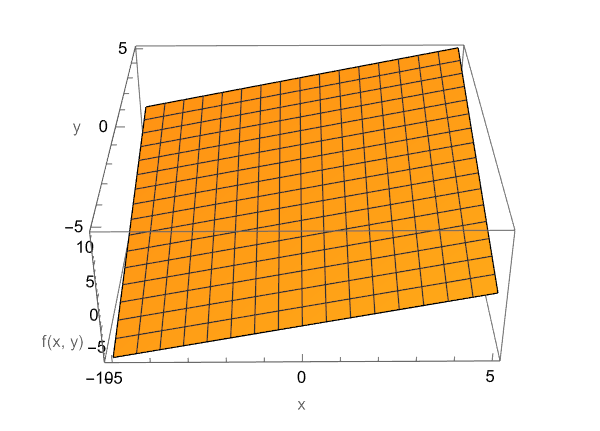
\includegraphics[width=0.7\linewidth]{Images/x+y}
			\caption{$f(x,y)=x+y$}
			\label{fig:xy}
		\end{figure}
		Let's see how the bivariate function $f(x, y) = x + y$ is related to the univariate functions $f(x) = x$ and $f(y) = y$.
		
		When we fix the value of $y$, say $y = y_0$, the function $f(x, y)$ becomes a univariate function in $x$: $f(x, y_0) = x + y_0$. This is essentially a vertical translation of the function $f(x) = x$ by a distance of $y_0$. In the 3D graph, this is represented by a line parallel to the $xz$-plane.
		Similarly, when we fix the value of $x$, say $x = x_0$, the function $f(x, y)$ becomes a univariate function in $y$: $f(x_0, y) = x_0 + y$. This is a vertical translation of the function $f(y) = y$ by a distance of $x_0$. In the 3D graph, this is represented by a line parallel to the $yz$-plane.
		When $y = 0$, $f(x, 0) = x$, which is the graph of the function $f(x) = x$. In the 3D graph, this is a line on the $xy$-plane.
		When $x = 0$, $f(0, y) = y$, which is the graph of the function $f(y) = y$. In the 3D graph, this is also a line on the $xy$-plane.
		The graphs of the functions $f(x) = x$ and $f(y) = y$ intersect on the $xy$-plane at the point $(0, 0)$, which corresponds to the point $(0, 0, 0)$ in the 3D graph.
		You can imagine that the graph of the function $f(x, y) = x + y$ is composed of countless lines parallel to the $xz$-plane and $yz$-plane, which correspond to the translations of $f(x) = x$ and $f(y) = y$ respectively. These lines form a plane in the 3D space.
		
		This plane can be seen as the result of translating $f(x) = x$ along the $y$-axis, or translating $f(y) = y$ along the $x$-axis. The combination of these two univariate functions in the 3D space forms the graph of the bivariate function $f(x, y) = x + y$.
	    \end{example}
	    
	    \begin{remark}
	    	Do not mix it up with function addition and multiplication earlier, because for the cases earlier, all functions are with respect to $x$, the same variable,
	    	while in this case a new variable is introduced.
	    \end{remark}
	    
	    
		We have worked out this example, however, here I'd like to give some extra knowledge on Cartesian product, especially its geometrical meaning. We just mentioned that two number set 
		will produce a set of ordered pairs with two elements, and in this case, we denote the set formed by Cartesian product of the same real number set as $\R^2$. Nevertheless, ordered pairs'
		elements are not always in pairs. We can even define an ordered pair of one single real number $(a)$, where $a \in \R$, or even three or more elements. We first examine $\R$ and $(a)$, 
		it is clear that $\R$ is just the set of real number that is already defined, while the ordered pair $(a)$ represents some $a\in \R$. Now we introduce another $b\in \R$ to
		form ordered pair $(a,b)$, and we have concluded that $(a,b) \in \R^2$. The process of developing $(a)$ to $(a,b)$,  is just creating a Cartesian product of real number set 
		to itself. To visualize this process, we need to find a suitable carrier for real number. We know that a real number could be infinitely huge or infinitely small, as there is no
		biggest or smallest real number (even though we haven't proven this, we just take it as common sense). We take some real number $-2 <r < 2$ as example. We can see that this interval is
		actually defined by a line on the Cartesian plane (or the Cartesian Coordinates). Since real number are infinite, so the whole set ordered pair $(a), a\in \R$, are defined in a line
		extending to both left and right-hand-side of the plane, giving us a whole line that extents forever.
		\begin{figure}[H]
			\centering
			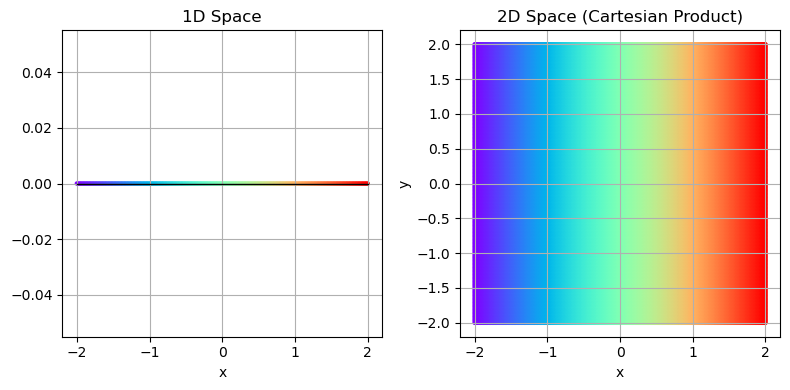
\includegraphics[width=0.8\linewidth]{Images/R^2}
			\caption{Visualization of $\R^1$ and $\R^2$}
			\label{fig:r2}
		\end{figure}
		Now we consider $(a,b)$, where both elements are from $\R$, so for the Cartesian products, we will get all possible combination of any $\R\times \R$. In this way, we can get a plane, just as
		shown in the graph. This is why call this system "Cartesian Coordinate". Naturally, we can also conclude that $\R^3 $ is a solid cubic in the 3D space.
		\begin{figure}[H]
			\centering
			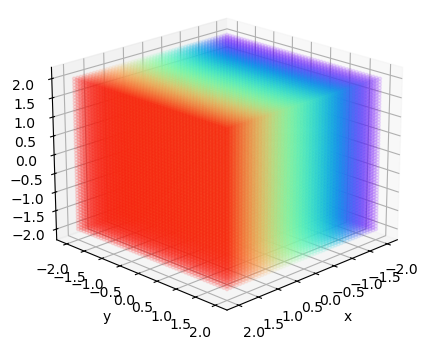
\includegraphics[width=0.7\linewidth]{Images/R^3}
			\caption[]{Visualization of $\R^3$}
			\label{fig:r3}
		\end{figure}
		But what about functions whose preimage are above $\R^3$? Sadly, there is no easy way to plot a function that are in 4D space, even though we can still use many techniques to analyze these
		high dimension functions, including function slicing. We will discuss $\R^n$ further in linear algebra and multivariable calculus. 
		
		Just now, we have somewhat shown another law about dimension or graphical representation of function.
		\begin{proposition}
			For any \textbf{n-variable function} with variables $x_1, x_2, \cdots, x_n$, for function $f(x_1,x_2,\cdots, x_n)$, ($x\in \R$), whose mapping is $\R \times \R \times \cdots \times \R = \R^n \to \R$.
			we need $n+1$ dimensions to plot a complete graph for the function. 
		\end{proposition}
		
		
		Additionally, $\R^n$ is defined as \textbf{The n-dimensional Euclidean Space}.
		\begin{definition}[The n-dimensional Euclidean Space]
		The n-dimensional Euclidean Space can be defined as the set of all real-valued functions defined on the index set $\{1, 2, \ldots, n\}$.
			\[\mathbb{R}^n = \{f \colon \{1, 2, \ldots, n\} \to \mathbb{R}\}\]
			
			where each function $f$ assigns a real number to each element of the index set $\{1, 2, \ldots, n\}$. We can represent these functions as n-tuples or vectors:
			
			\[f = (f(1), f(2), \ldots, f(n)) = (x_1, x_2, \ldots, x_n)\]
			
			where $x_i = f(i)$ for $i = 1, 2, \ldots, n$. Thus, each point in $\mathbb{R}^n$ can be identified with an n-tuple of real numbers $(x_1, x_2, \ldots, x_n)$.
			
			The set $\mathbb{R}^n$ is equipped with various algebraic and geometric structures, such as vector addition, scalar multiplication, and an inner product, which make it a real vector space of dimension $n$. Don't worry if you are confused by this, we will explore this topic further in linear algebra and other topics.
		\end{definition}
		
\subsection{Partial and Total Function}
Now we will introduce some ways to categorize functions. Earlier, we have discussed many functions where $f: \R \to \R$, but functions cannot always 
have a domain in a complete set. So we first introduce the idea of partial function.
\begin{definition}[Partial Function]
	A partial function from a set $A$ to a set $B$ is a function $f$ that satisfies the following conditions:
	\begin{enumerate}
		\item The domain of $f$, denoted by $\text{dom}(f)$, is a subset of $A$, i.e., $\text{dom}(f) \subseteq A$.
		\item For each $x \in \text{dom}(f)$, there is a unique $y \in B$ such that $f(x) = y$.
	\end{enumerate}
	
	In other words, a partial function is a function that may not be defined for all elements of its source set. Partial functions allow some input values to have no corresponding output values.
\end{definition}
\begin{example}
	Consider the function $f: \mathbb{R} \to \mathbb{R}$ defined as:
	$$
	f(x) = \begin{cases}
		\frac{1}{x}, & \text{if } x \neq 0 \\
		\text{undefined}, & \text{if } x = 0
	\end{cases}
	$$
	This function $f$ is a partial function because it is not defined for $x = 0$. The domain of $f$ is the set of all real numbers except zero, i.e., $\text{dom}(f) = \mathbb{R} \setminus {0}$.
\end{example}

By analogy, we can define total function as follows.
\begin{definition}[Total Function]
	A total function from a set $A$ to a set $B$ is a function $f$ that satisfies the following conditions:
	\begin{enumerate}
		\item The domain of $f$, denoted by $\text{dom}(f)$, is equal to $A$, i.e., $\text{dom}(f) = A$.
		\item For each $x \in A$, there is a unique $y \in B$ such that $f(x) = y$.
	\end{enumerate}
	
	In other words, a total function is a function that is defined for all elements of its source set. Every input value of a total function has a unique corresponding output value.
\end{definition}
\begin{example}
	Consider the function $g: \mathbb{R} \to \mathbb{R}$ defined as:
	$$
	g(x) = x^2
	$$
	
	This function $g$ is a total function because it is defined for all real numbers. The domain of $g$ is the entire set of real numbers, i.e., $\text{dom}(g) = \mathbb{R}$. For any input value $x \in \mathbb{R}$, the function $g$ assigns the unique output value $x^2$.
	
	A total function is a special case of a partial function where the domain is equal to the source set.
	
\end{example}

Another thing that worth discussing is that, earlier, we introduced function slicing that reduce the number of variable of a function. Function slicing has 
much to do with partial function.
\begin{proposition}[Function Slicing is Always a Partial Function]
	Function slicing is a technique that involves restricting the domain of a function to a specific subset. Given a function $f: A \to B$ and a subset $C \subseteq A$, the slice of $f$ over $C$, denoted by $f|_C$, is defined as:
	$$
	f|_C(x) = \begin{cases}
		f(x), & \text{if } x \in C \\
		\text{undefined}, & \text{if } x \notin C
	\end{cases}
	$$
	The function $f|_C$ has the same output values as $f$ for inputs in $C$, but it is undefined for inputs not in $C$.
	
	If the original function $f$ is a total function, then the slice $f|_C$ is a partial function, unless $C = A$. In the case where $C = A$, the slice $f|_C$ is the same as the original function $f$ and remains a total function.
	
	On the other hand, if the original function $f$ is already a partial function, then the slice $f|_C$ is also a partial function, regardless of the choice of $C$.
\end{proposition}







\subsection{Injective, Surjective, and Bijective Function}
We have known that functions are actually reflection from one set to the other set. We will look into several special mapping.

\begin{definition}[Injective Function]
    A function \( f: A \to B \) is called \emph{injective} (or \emph{one-to-one}) if every element of the codomain \( B \) is mapped by at most one element of the domain \( A \). For example, the function \( f(x) = 2x \) from \( \mathbb{R} \) to \( \mathbb{R} \) is injective because each value of \( f(x) \) is produced by exactly one value of \( x \).
\end{definition}

\begin{definition}[Surjective Function]
    A function is \emph{surjective} (or \emph{onto}) if every element of the codomain \( B \) is mapped by at least one element of the domain \( A \). For instance, the function \( g(x) = \sin(x) \) from \( \mathbb{R} \) to \( [-1, 1] \) is surjective because every value in \( [-1, 1] \) is the sine of some real number \( x \).
\end{definition}

\begin{definition}[Bijective Function]
    A function is \emph{bijective} if it is both injective and surjective, which means there is a perfect "pairing" between the sets: every element of \( A \) is paired with a unique element of \( B \), and every element of \( B \) is paired with a unique element of \( A \). An example of a bijective function is the identity function \( i(x) = x \) from \( \mathbb{R} \) to \( \mathbb{R} \).
\end{definition}

\begin{figure}[H]
    \centering
    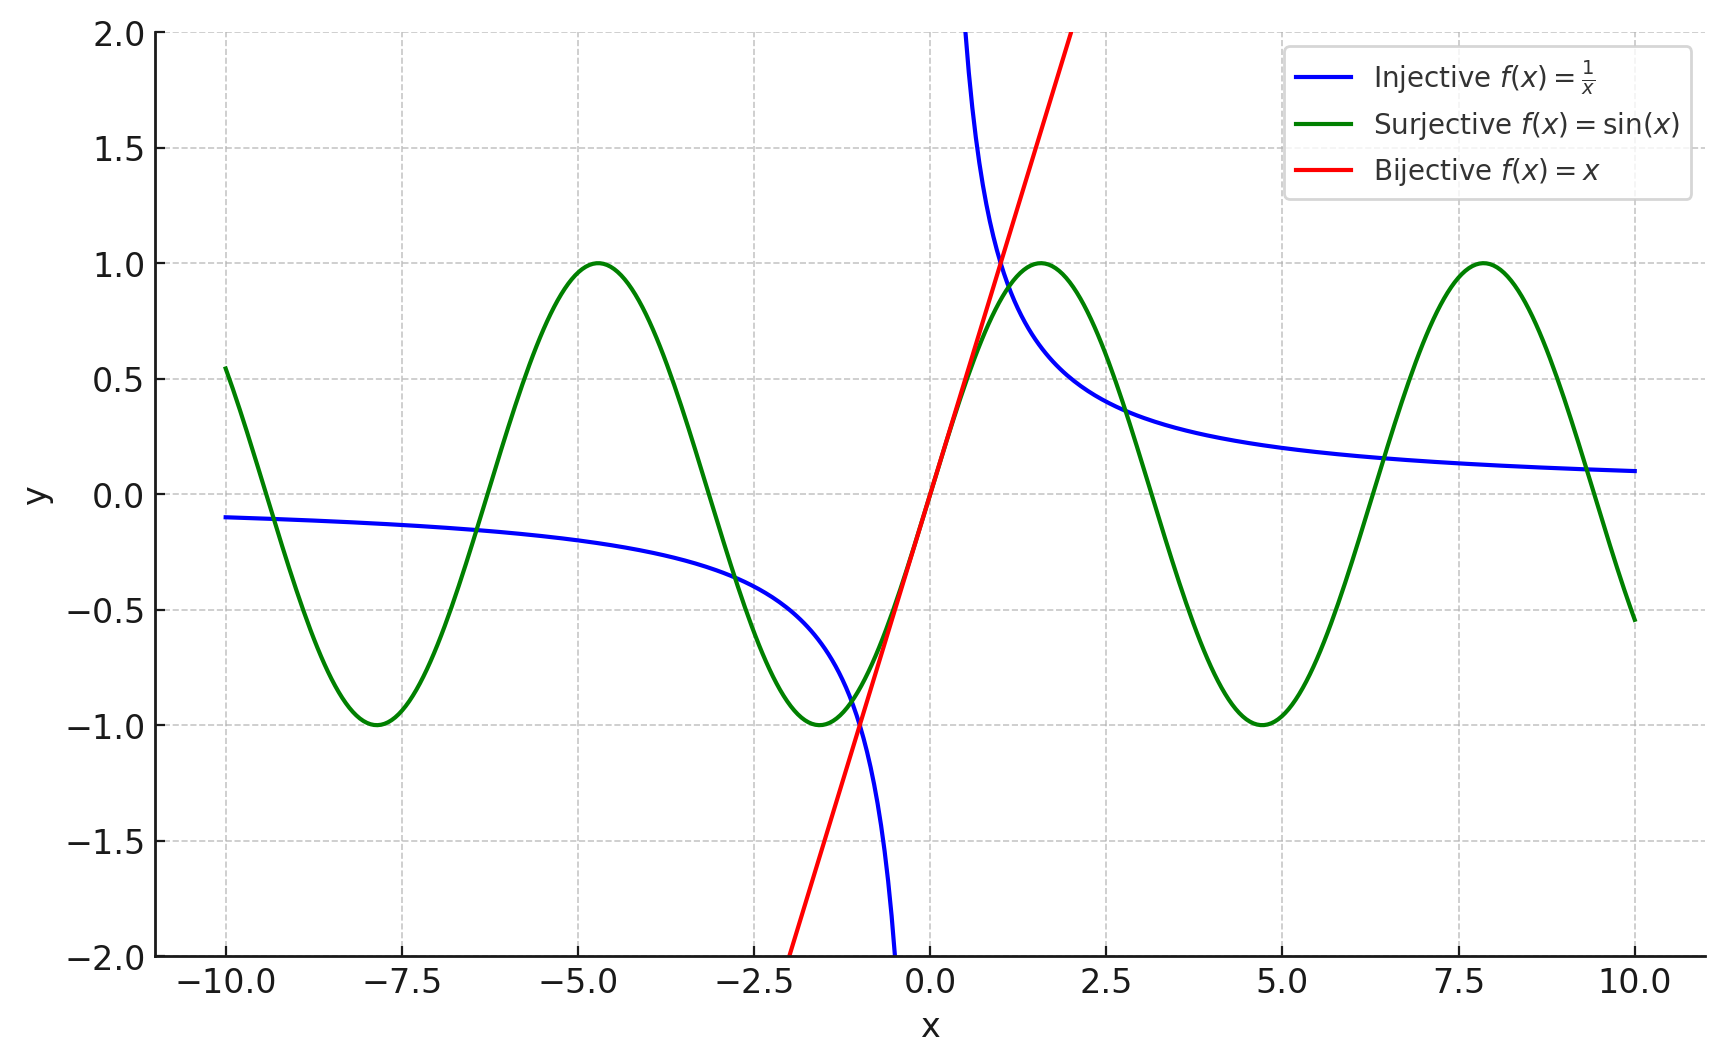
\includegraphics[width=0.75\linewidth]{Images/func.jpg}
    \caption{Examples of Special Mappings}
    \label{fig:fuc}
\end{figure}

Examine the figure \autoref{fig:fuc}, where one example of each type of function is shown. Fundamentally, when we define these functions, only two properties are involve:
\begin{itemize}
    \item A: It the mapping retrievable? (for every value in the image, we can find where it is from without any confusion.
    \item B: Is the mapping is full comparing to the preimage?(Whether every value in the preimage has a mapping to the image)
\end{itemize}
If A is satisfied, we call it injective function.

If B is satisfied, we call it surjective function.

If both A and B are satisfied, we say the function is bijective.

Using $A$, $B$, and $C$ to denote the set of injective, surjective, and bijective function respectively, it is therefore that :

    $$A\cap B = C$$

Which means that if a function is injective and surjective in the same time, it is bijective. 

Additionally, we need to distinguish bijective function with well-defined function.
\begin{definition}[Well-defined Function]
	A function \( f: A \rightarrow B \) is said to be \emph{well-defined} if for every element \( a \) 
	in the domain \( A \), there is a unique element \( b \) in the codomain \( B \) such that \( f(a) = b \). 
	This means that the function assigns exactly one output to each input. A well-defined function does not 
	assign multiple outputs to a single input, and every input for which the function is defined has an 
	output.
\end{definition}
\begin{remark}
	While all bijective functions are well-defined, not all well-defined functions are bijective. 
	Being well-defined is a minimal requirement for being a function at all. A well-defined function may 
	fail to be bijective if it is not injective, allowing different inputs to have the same output, or if 
	it is not surjective, meaning that some elements in the codomain do not correspond to any input from 
	the domain. Thus, while bijectivity implies a specific one-to-one correspondence between the entire 
	domain and codomain, well-definedness merely ensures that the function is consistently defined across 
	its domain.
\end{remark}
And these will be all we need to know about function for now, since the rest of the properties will be discussed in single-variable calculus. This section aims only introduce the idea of injectivity, surjectivity, and bijectivity.

\subsection{Exercises}

\begin{exercise}
	Let $f : \{0, 1\} \times \mathcal{P}(\mathbb{Z}) \to \mathbb{N}$ be a function. Which of the following correctly gives an example of an element from its domain and an element from its codomain?
	\begin{enumerate}
		\item $(8, -7)$ is an element of the domain and ${1, 9, 85}$ is an element of the codomain.
		\item $1$ is an element of the domain and ${6, 8}$ is an element of the codomain.
		\item ${0, 14}$ is an element of the domain and $19$ is an element of the codomain.
		\item $(1, \{-3, 6\})$ is an element of the domain and $9$ is an element of the codomain.
	\end{enumerate}
\end{exercise}
\begin{solution}
	Let's break down the domain and codomain of the function $f$:
	
	\begin{itemize}
		\item The domain of $f$ is ${0, 1} \times \mathcal{P}(\mathbb{Z})$, which means it consists of ordered pairs $(a, B)$, where $a$ is either $0$ or $1$, and $B$ is a subset of the set of integers $\mathbb{Z}$.
		\item The codomain of $f$ is $\mathbb{N}$, which is the set of natural numbers.
	\end{itemize}
	
	Now, let's examine each choice:
	
	\begin{enumerate}
		\item $(8, -7)$ is not an element of the domain because $8 \notin \{0, 1\}$, and $-7$ is not a subset of $\mathbb{Z}$. $\{1, 9, 85\}$ is a subset of $\mathbb{N}$, but not an element of $\mathbb{N}$.
		\item $1$ is an element of $\{0, 1\}$, but not an element of $\{0, 1\} \times \mathcal{P}(\mathbb{Z})$. $\{6, 8\}$ is a subset of $\mathbb{N}$, but not an element of $\mathbb{N}$.
		\item $\{0, 14\}$ is not an element of $\{0, 1\} \times \mathcal{P}(\mathbb{Z})$ because it is not an ordered pair. $19$ is an element of $\mathbb{N}$.
		\item $(1, \{-3, 6\})$ is an element of $\{0, 1\} \times \mathcal{P}(\mathbb{Z})$ because $1 \in \{0, 1\}$ and $\{-3, 6\} \subseteq \mathbb{Z}$. $9$ is an element of $\mathbb{N}$.
	\end{enumerate}
	
	Therefore, the correct answer is 4.
\end{solution}
\begin{exercise}
	Determine whether the rules below define functions from $\mathbb{R}$ to $\mathbb{R}$.
	\begin{enumerate}
		\item[a)] \( f(x) = 
		\begin{cases} 
		|x - 1| & \text{if } x < 4 \\
		|x| - 1 & \text{if } x > 2.
		\end{cases} \)
		
		\item[b)] \( f(x) = 
		\begin{cases} 
		|x - 1| & \text{if } x < 2 \\
		|x| - 1 & \text{if } x > -1.
		\end{cases} \)
		
		\item[c)] \( f(x) = 
		\begin{cases} 
		\frac{(x + 3)^2 - 9}{x} & \text{if } x \neq 0 \\
		6 & \text{if } x = 0.
		\end{cases} \)
		
		\item[d)] \( f(x) = 
		\begin{cases} 
		\frac{(x + 3)^2 - 9}{x} & \text{if } x > 0 \\
		x + 6 & \text{if } x < 7.
		\end{cases} \)
		
		\item[e)] \( f(x) = 
		\begin{cases} 
		\sqrt{x^2} & \text{if } x \geq 2 \\
		x & \text{if } 0 \leq x \leq 4 \\
		-x & \text{if } x < 0.
		\end{cases} \)
	\end{enumerate}
\end{exercise}
\begin{remark}
	You only need to check whether the domain covers the whole $\R$.
\end{remark}
\begin{exercise}
    Determine the images of the functions \( f: \mathbb{R} \rightarrow \mathbb{R} \) defined as follows:
    \begin{enumerate}
        \item[a)] \( f(x) = \frac{x^2}{1 + x^2} \).
        \item[b)] \( f(x) = \frac{x}{1 + |x|} \).
    \end{enumerate}
\end{exercise}
\begin{solution}
    We analyze the function \( f(x) = \frac{x^2}{1 + x^2} \):
    \begin{itemize}
        \item This function is defined for all \( x \in \mathbb{R} \).
        \item For \( x = 0 \), \( f(0) = 0 \).
        \item For \( x \neq 0 \), \( f(x) \) is always positive.
        \item As \( x \) approaches infinity, \( f(x) \) approaches 1.
    \end{itemize}
    Thus, the image of \( f \) is \( (0, 1] \).
    

    We analyze the function \( f(x) = \frac{x}{1 + |x|} \):
    \begin{itemize}
        \item This function is defined for all \( x \in \mathbb{R} \).
        \item For \( x > 0 \), as \( x \) increases, \( f(x) \) approaches 1.
        \item For \( x < 0 \), as \( x \) decreases, \( f(x) \) approaches -1.
    \end{itemize}
    Thus, the image of \( f \) is \( (-1, 1) \).
    \end{solution}

\begin{exercise}
	Let $f:\mathbb{Z}^+\times\mathbb{Z}^+\to\mathbb{Z}$ be the function defined by $f((a,b))=\gcd(a,b)+b$ where $\mathbb{Z}^+$ is the set of positive integers and $\gcd(a,b)$ is the greatest common divisor of $a$ and $b$.
	Is this a one-to-one (bijective) function? What is the image of the function?
\end{exercise}
\begin{solution}
	Take $(a_1, b_1) = (2, 2)$ and $(a_2, b_2) = (1, 3)$. Both $(2, 2)$ and $(1, 3)$ are elements of the domain $\mathbb{Z}^+ \times \mathbb{Z}^+$.
	
	Now, let's calculate $f((2, 2))$ and $f((1, 3))$:
	
	$f((2, 2)) = \gcd(2, 2) + 2 = 2 + 2 = 4$
	$f((1, 3)) = \gcd(1, 3) + 3 = 1 + 3 = 4$
	
	As we can see, $f((2, 2)) = f((1, 3)) = 4$, even though $(2, 2) \neq (1, 3)$. This demonstrates that $f$ is not one-to-one, as there exist distinct elements in the domain that map to the same element in the codomain.
	
	Now, let's determine the image of $f$. The image of a function is the set of all elements in the codomain that are mapped to by at least one element in the domain.
	
	Observe that for any $(a, b) \in \mathbb{Z}^+ \times \mathbb{Z}^+$:
	
	$\gcd(a, b) \geq 1$, because the greatest common divisor of two positive integers is always a positive integer.
	$b \geq 1$, because $b$ is a positive integer.
	Therefore, $f((a, b)) = \gcd(a, b) + b \geq 1 + 1 = 2$.
	
	This means that the smallest possible value of $f((a, b))$ is 2, and there is no upper limit on the value of $f((a, b))$ as $b$ can be arbitrarily large.
	
	Thus, the image of $f$ is the set ${x : x \in \mathbb{Z} \text{ and } x \geq 2}$, which is the set of all integers greater than or equal to 2.
	
	In conclusion, $f$ is not a one-to-one function, and its image is ${x : x \in \mathbb{Z} \text{ and } x \geq 2}$.
\end{solution}

\begin{exercise}
	Considering $X=\{1,2,3\}$ and $Y=\{a,b\}$. How to define a total function $f: X\to Y$?
	How many are there? List all the total functions. Also try to find the way to calculate
	the number of total functions obtained by $X$ and $Y$ with respect to $|X|, |Y|$.
\end{exercise}
\begin{solution}
	To obtain a total function, we must make sure that the preimage is exactly $X=\{1,2,3\}$, so we can pick which ever combinations of members of $Y$, so we have
	$(a, a, a)$,
	$(a, a, b)$,
	$(a, b, a)$,
	$(a, b, b)$,
	$(b, a, a)$,
	$(b, a, b)$,
	$(b, b, a)$,
	$(b, b, b)$.
	There are 8 total functions from $X$ to $Y$.
	 The number of total functions can be calculated using the formula $|Y|^{|X|}$, which in this case is $2^3 = 8$.
\end{solution}
\begin{exercise}
	Let $f$ and $g$ be the following functions.\\ $f:\mathcal{P}(\{1,2,3,4\})\to\mathcal{P}(\{1,2,3,4\})$ defined by $f(X)=\{1,2,3,4\}-X$.
	
	\noindent $g:\mathcal{P}(\{1,2,3,4\})\cdot\to\{0,1,2,3,4\}$ defined by $g(X)=|X|$.
	Discuss the existence of $f(f(x)), f(g(x)), g(f(x)), and g(g(x))$. If any
	of them exists, give a example.
\end{exercise}
\begin{solution}
	\textbf{1. $f(f(x))$:}
	$f(f(x))$ exists for all $x \in \mathcal{P}({1,2,3,4})$ because the codomain of $f$ is the same as its domain. This means that for any $x \subseteq {1,2,3,4}$, $f(x) \subseteq {1,2,3,4}$, so $f(f(x))$ is well-defined.
	
	Example:
	Let $x = {1,3}$. Then:
	\begin{align*}
		f(x) &= {1,2,3,4} - {1,3} = {2,4} \\
		f(f(x)) &= f({2,4}) = {1,2,3,4} - {2,4} = {1,3}
	\end{align*}
	
	\textbf{2. $f(g(x))$:}
	$f(g(x))$ does not exist because the codomain of $g$ is ${0,1,2,3,4}$, which is not a subset of the domain of $f$, $\mathcal{P}({1,2,3,4})$. Therefore, $g(x)$ is not a valid input for $f$.
	
	\textbf{3. $g(f(x))$:}
	$g(f(x))$ exists for all $x \in \mathcal{P}({1,2,3,4})$ because the codomain of $f$ is $\mathcal{P}({1,2,3,4})$, which is the domain of $g$. This means that for any $x \subseteq {1,2,3,4}$, $f(x) \subseteq {1,2,3,4}$, so $g(f(x))$ is well-defined.
	
	Example:
	Let $x = {2,3}$. Then:
	\begin{align*}
		f(x) &= {1,2,3,4} - {2,3} = {1,4} \\
		g(f(x)) &= g({1,4}) = |{1,4}| = 2
	\end{align*}
	
	\textbf{4. $g(g(x))$:}
	$g(g(x))$ does not exist because the codomain of $g$ is ${0,1,2,3,4}$, which is not a subset of the domain of $g$, $\mathcal{P}({1,2,3,4})$. Therefore, $g(x)$ is not a valid input for $g$.
	
	In summary, $f(f(x))$ and $g(f(x))$ exist for all $x \in \mathcal{P}({1,2,3,4})$, while $f(g(x))$ and $g(g(x))$ do not exist.
\end{solution}

\begin{exercise}
	We have discussed $\R^1$ to $\R^n$ in this section. Try to postulate that
	whether $R^0$ exists? If it exists, can it be defined by Cartesian Product.
	Try to prove your conclusion by deduction, and explain how can we visualize it, and
	is it necessary to visualize it in Cartesian Coordinate system.
	\begin{remark}
		Deduction is also known as "inverse induction".
	\end{remark}
\end{exercise}
\begin{proof}
	First, let's recall the definition of the Cartesian product for a finite collection of sets $A_1, A_2, \ldots, A_n$:
	
	\begin{align*}
		A_1 \times A_2 \times \cdots \times A_n = {(a_1, a_2, \ldots, a_n) \mid a_1 \in A_1, a_2 \in A_2, \ldots, a_n \in A_n}
	\end{align*}
	
	Now, consider the case where $n = 0$. We have an empty collection of sets, denoted by $\emptyset$. The Cartesian product of an empty collection of sets is defined as:
	
	\begin{align*}
		\prod_{i \in \emptyset} A_i = {()}
	\end{align*}
	
	This is a singleton set containing the empty tuple $()$. The empty tuple is a tuple with no components and is denoted by $()$.
	
	By definition, $\mathbb{R}^n$ is the Cartesian product of $n$ copies of $\mathbb{R}$:
	
	\begin{align*}
		\mathbb{R}^n = \underbrace{\mathbb{R} \times \mathbb{R} \times \cdots \times \mathbb{R}}_{n \text{ times}}
	\end{align*}
	
	When $n = 0$, we have:
	
	\begin{align*}
		\mathbb{R}^0 = \prod_{i \in \emptyset} \mathbb{R} = {()}
	\end{align*}
	
	Therefore, $\mathbb{R}^0$ exists and is equal to the singleton set containing the empty tuple $()$.
	
	\textbf{Visualization:}
	As mentioned earlier, visualizing $\mathbb{R}^0$ is not necessary, as it is a singleton set containing only the empty tuple. However, if we were to visualize it, it would be represented by a single point in a 0-dimensional space.
	
	In the Cartesian coordinate system, $\mathbb{R}^1$ is represented by a line, $\mathbb{R}^2$ by a plane, and $\mathbb{R}^3$ by a 3-dimensional space. As the dimension increases, the visualization becomes more complex. For $\mathbb{R}^0$, there are no axes to represent it in the Cartesian coordinate system, as it is a 0-dimensional space.
	
	\textbf{Conclusion:}
	$\mathbb{R}^0$ exists and can be defined as the Cartesian product of zero copies of $\mathbb{R}$, resulting in a singleton set containing the empty tuple $()$. While it is not necessary to visualize $\mathbb{R}^0$ in the Cartesian coordinate system, it can be thought of as a single point in a 0-dimensional space.
\end{proof}

\begin{exercise}
	If $f:A\to B$ and $g:B\to C$ are bijections (both injections and surjections), prove that 
	$g\circ f:A\to C$ is also a bijection.
\end{exercise}
\begin{proof}
	We aim to prove that the composition of two bijective functions is also a bijection.

	Let \(f: A \to B\) and \(g: B \to C\) be bijections. We need to show that \(g \circ f: A \to C\) is both an injection and a surjection.

	Assume \(x_1, x_2 \in A\) and \(g(f(x_1)) = g(f(x_2))\). Since \(g\) is an injection, if \(g(y_1) = g(y_2)\) then \(y_1 = y_2\) for any \(y_1, y_2 \in B\), which implies \(f(x_1) = f(x_2)\). Furthermore, since \(f\) is also an injection, \(x_1 = x_2\). Hence, \(g \circ f\) is an injection.

	Let \(z \in C\). Since \(g\) is a surjection, there exists \(y \in B\) such that \(g(y) = z\). Similarly, since \(f\) is a surjection, there exists \(x \in A\) such that \(f(x) = y\). Therefore, for \(z \in C\), there exists \(x \in A\) such that \(g(f(x)) = z\). Thus, \(g \circ f\) is a surjection.

	Combining both, we conclude that \(g \circ f\) is a bijection.
\end{proof}

\begin{exercise}
	is the inverse proposition of last statement true, if so prove it.
\end{exercise}
\begin{proof}
	We can use proof by contradiction here.\\
	Suppose that $g: A\to B$ and $f: B\to C, $ so that $f\circ g: A\to C$ . We will prove that if 
	$f\circ g$ is one-to-one, then $g$ is also one-to-one, so not only is the answer to the question “yes”. 
	Suppose that $g$ were not one-to-one. By definition this means that there are distinct elements 
	$a_1$ and $a_2$ in $A$ such that $g( a_1) = g( a_2) .$ Then certainly $f(g(a_1))=f(g(a_2))$, which is 
	the same statement as $(f\circ g)(a_1)=(f\circ g)(a_2).$ By definition this means that $f\circ g$ is not
	one-to-one, and our proof is complete.

\end{proof}
\begin{exercise}
	Let \( f \) be a function with domain \( \mathcal{D} \) and \( f(S) = \{ f(x) : x \in S \} \) for any subset \( S \) of \( \mathcal{D} \). Suppose \( C \) and \( D \) are subsets of \( \mathcal{D} \).
\begin{enumerate}
    \item[a)] Prove that \( f(C \cup D) \subseteq f(C) \cup f(D) \).
    \item[b)] Give an example where equality does not hold in part (a).
\end{enumerate}
\end{exercise}
\begin{solution}
	Below is solution for a).
	\begin{proof}
		Take any element \( y \in f(C \cup D) \). By definition of \( f(S) \), there exists an 
		\( x \in C \cup D \) such that \( f(x) = y \). Since \( x \) is in the union \( C \cup D \), 
		\( x \) must be in either \( C \) or \( D \). If \( x \in C \), then \( y = f(x) \in f(C) \). 
		Similarly, if \( x \in D \), then \( y = f(x) \in f(D) \). Therefore, in either case, 
		\( y \in f(C) \cup f(D) \), proving that \( f(C \cup D) \subseteq f(C) \cup f(D) \).
	\end{proof}
	Below is an example that the inequality holds.
	\begin{align*}
		f: \mathbb{R} \to \mathbb{R}, \quad f(x) &= x^2 \\
		C &= \{-1, 1\} \\
		D &= \{0, 2\} \\
		f(C) &= \{f(x) \mid x \in C\} = \{1\} \\
		f(D) &= \{f(x) \mid x \in D\} = \{0, 4\} \\
		f(C) \cup f(D) &= \{0, 1, 4\} \\
		f(C \cup D) &= \{f(x) \mid x \in C \cup D\} = \{0, 1, 4, 9\} \\
		\therefore f(C \cup D) &\neq f(C) \cup f(D)
	\end{align*}
	The equality does not hold when the function f is not injective,
	meaning that it maps distinct elements in the domain to the same element in the codomain. 
\end{solution}

\begin{exercise}
	Determine whether \( f: \mathbb{Z} \times \mathbb{Z} \rightarrow \mathbb{Z} \) is onto if
	\begin{enumerate}[label=(\alph*)]
		\item \( f(m, n) = 2m - n. \)
		\item \( f(m, n) = m^2 - n^2. \)
		\item \( f(m, n) = m + n + 1. \)
		\item \( f(m, n) = |m| - |n|. \)
		\item \( f(m, n) = m^2 - 4. \)
	\end{enumerate}
	\end{exercise}
	
	\begin{solution} 
	\begin{enumerate}[label=(\alph*)]
		\item This is clearly onto, since \( f(0, -n) = n \) for every integer \( n \).
		\item This is not onto, since, for example, \( 2 \) is not in the range. To see this, if \( m^2 - n^2 = (m - n)(m + n) = 2 \), then \( m \) and \( n \) must have the same parity (both even or both odd). In either case, both \( m - n \) and \( m + n \) are then even, so this expression is divisible by 4 and hence cannot equal 2.
		\item This is clearly onto, since \( f(0, n - 1) = n \) for every integer \( n \).
		\item This is onto. To achieve negative values we set \( m = 0 \), and to achieve nonnegative values we set \( n = 0 \).
		\item This is not onto, for the same reason as in part (b). In fact, the range here is clearly a subset of the range in that part.
	\end{enumerate}
	\end{solution}

	\begin{exercise}
		Let \( f \) be a function from the set \( A \) to the set \( B \). Let \( S \) and \( T \) be subsets of \( A \). Show that
		\begin{enumerate}[label=(\alph*)]
			\item \( f(S \cup T) = f(S) \cup f(T) \).
			\item \( f(S \cap T) \subseteq f(S) \cap f(T) \).
		\end{enumerate}
		\end{exercise}
		
		\begin{solution}
		\begin{enumerate}[label=(\alph*)]
			\item We need to show two inclusions:
			\begin{itemize}
				\item Suppose \( b \in f(S \cup T) \). This implies \( b = f(a) \) for some \( a \in S \cup T \). Thus, \( a \in S \) or \( a \in T \), and consequently, \( b \in f(S) \) or \( b \in f(T) \). Hence, \( b \in f(S) \cup f(T) \).
				
				\item Conversely, assume \( b \in f(S) \cup f(T) \). Then either \( b \in f(S) \) or \( b \in f(T) \), which means there exists an \( a \in S \) or \( a \in T \) such that \( b = f(a) \). Thus, \( a \in S \cup T \) and \( b \in f(S \cup T) \).
			\end{itemize}
			This shows that \( f(S \cup T) = f(S) \cup f(T) \), completing the proof.
		
			\item To prove the subset relation:
			\begin{itemize}
				\item Let \( b \in f(S \cap T) \). Then \( b = f(a) \) for some \( a \in S \cap T \). This means \( a \in S \) and \( a \in T \), hence \( b \in f(S) \) and \( b \in f(T) \). Therefore, \( b \in f(S) \cap f(T) \).
			\end{itemize}
			This establishes that \( f(S \cap T) \subseteq f(S) \cap f(T) \), as desired.
		\end{enumerate}
		\end{solution}

		\begin{exercise}
			Show that a partial function from \( A \) to \( B \) can be viewed as a function \( f^* \) from \( A \) to \( B \cup \{u\} \), where \( u \) is not an element of \( B \) and
			\[
			f^*(a) = 
			\begin{cases} 
			f(a) & \text{if } a \text{ belongs to the domain of definition of } f \\
			u & \text{if } f \text{ is undefined at } a.
			\end{cases}
			\]
			\end{exercise}
			
			\begin{solution}
			To show that a partial function \( f \) from \( A \) to \( B \) can be extended to a total function \( f^* \) from \( A \) to \( B \cup \{u\} \), we need to verify that for every element \( a \) in \( A \), the function \( f^* \) assigns exactly one element in \( B \cup \{u\} \).
			
			Consider any element \( a \) in \( A \). There are two possibilities:
			
			\begin{enumerate}
				\item If \( a \) is in the domain of definition of \( f \), then by the definition of \( f \), there is an associated element \( f(a) \) in \( B \). In this case, we define \( f^*(a) = f(a) \). Since \( f(a) \) is an element of \( B \), and \( B \) is a subset of \( B \cup \{u\} \), \( f^*(a) \) is an element of \( B \cup \{u\} \).
				
				\item If \( a \) is not in the domain of \( f \), which means \( f \) is undefined at \( a \), we assign a special element \( u \) that is not in \( B \) to \( a \). Specifically, we define \( f^*(a) = u \). By the choice of \( u \), we ensure that \( f^*(a) \) is in \( B \cup \{u\} \).
			\end{enumerate}
			
			In both cases, \( f^*(a) \) is a well-defined element of \( B \cup \{u\} \). Furthermore, the definition of \( f^* \) is such that each \( a \) in \( A \) is associated with exactly one element in \( B \cup \{u\} \), making \( f^* \) a total function. Therefore, \( f^* \) satisfies the definition of a function and extends \( f \) to the entire set \( A \) by assigning \( u \) where \( f \) is undefined.
			
			Thus, every partial function \( f: A \rightarrow B \) can indeed be considered a total function \( f^*: A \rightarrow B \cup \{u\} \) with the addition of a special element \( u \) to handle the undefined cases in \( f \).
			\end{solution}

			\begin{remark}
				The extension of a partial function \( f: A \rightarrow B \) to a total function \( f^*: A \rightarrow B \cup \{u\} \) relates closely to the concept of function slicing presented in Proposition 2.2 of the book. Function slicing involves restricting the domain of a function to a subset \( C \subseteq A \), whereas extending a partial function involves expanding the codomain to include an element \( u \) that handles undefined cases.
				
				In essence, slicing a total function can create a partial function \( f|_C \) which is only defined for inputs in subset \( C \). Extending a partial function \( f \) to \( f^* \) can be viewed as reversing this process, by adding an element to the codomain for the undefined cases, thereby making it total. 
				
				The slice \( f|_C \) has the same output values as \( f \) for inputs in \( C \), and is undefined for inputs not in \( C \). Similarly, \( f^* \) maintains the output values of \( f \) for inputs where \( f \) is defined and assigns the value \( u \) for inputs where \( f \) is not defined. Both processes — slicing and extending — are techniques to manipulate the domain and codomain of functions to achieve desired properties of partiality or totality.
			\end{remark}			
%------------------------------------------------
\section{Summation}
Before we move on to the most important part of this chapter, sequence, we use this section to introduce a prerequisite for studying its properties. We introduce the Sigma sign.

In earlier chapters, we have seen exercises such as finding the expression of the sum of the first nth positive integer:
$$1 + 2 + \dots + (n-1) + (n)= \frac{n(n+1)}{2}$$ 
From now on, we will use the sigma notation to deal with the summation of numbers. Such as:
\subsection{Sigma Notation}
\begin{notation}[Sigma Notation]
    \[
\sum_{i=1}^{n} i = \frac{n(n + 1)}{2}
    \]
\end{notation}
Where $i$ is quite similar to iterator, or sometimes we also call counter in programming languages, and $n$ refers to the condition of termination. The expression right after the sigma sign is called \textbf{summand}.

Actually, this is not the only way to express summation, it is also equivalent to:
\[\sum_{1\leq i\leq n} i = \frac{n(n+1)}{2}\]

Also, like what we do for set, we can also write sigma notation using description, such as: 
\[
\sum_{1 \leq k \leq 100} k^2
\]

\( k \) is odd

\subsection{Properties and Techniques of Sigma Notation}
This part of the section shows how we can handle summation expressions.
One of the greatest convenience of sigma notation is that every expression is adjustable, we can change the variable as what we prefer as in the following example.
\begin{example} \label{exp:siginvariance}
 \[
\sum_{1 \leq k \leq n} a_k = \sum_{1 \leq k+1 \leq n} a_{k+1}
\]
\end{example}
This technique has a significant effect to some mathematical proofs.
Another points to keep in mind is that: always make the expression simple in terms of upper and lower boundary.
\begin{example}
    Examine this expression: 
    \[\sum_{k=0}^{n} k(k-1)(k-n)\]
    The sum when k equals to 0, 1, and $n$ is 0. In this case we cannot say it is a good expression, as what we want is the sum it self, while 0 does not matter for us. Therefore, we just fine-tune it to:
    \[\sum_{k=2}^{n-1} k(k-1)(k-n)\]
    This makes it concise and clear.
\end{example}

\subsubsection{Manipulation of Sigma Notation}
For a set \( K \), the following summation properties hold. Let \( c \) be a constant, and \( a_k \), \( b_k \) be sequences indexed by \( K \):

\begin{equation}
    \sum_{k \in K} c a_k = c \sum_{k \in K} a_k \quad \text{(Distributive Law)}
    \label{eq:constant_factor}
\end{equation}

\begin{equation}
    \sum_{k \in K} (a_k + b_k) = \sum_{k \in K} a_k + \sum_{k \in K} b_k \quad \text{(Associative Law)}
    \label{eq:summation_of_sums}
\end{equation}

\begin{equation}
    \sum_{k \in K} a_k = \sum_{p(k) \in K} a_{p(k)} \quad \text{(Commutative Law, as in example \autoref{exp:siginvariance})} 
    \label{eq:permutation_invariance}
\end{equation}
The proof is attached below.

\textbf{Proof of Constant Factor Law:}

Let \( c \) be a constant and \( a_k \) be a sequence indexed by a finite set \( K \). We want to show that \( \sum_{k \in K} c a_k = c \sum_{k \in K} a_k \).

By the definition of summation and the distributive property of multiplication over addition, we have:
\begin{equation}
    \sum_{k \in K} c a_k = c a_1 + c a_2 + \ldots + c a_n = c (a_1 + a_2 + \ldots + a_n) = c \sum_{k \in K} a_k.
\end{equation}
This concludes the proof of the constant factor law.

\textbf{Proof of Summation of Sums Law:}

Let \( a_k \) and \( b_k \) be sequences indexed by a finite set \( K \). We want to show that \( \sum_{k \in K} (a_k + b_k) = \sum_{k \in K} a_k + \sum_{k \in K} b_k \).

By the definition of summation and the associative and commutative properties of addition, we have:
\begin{equation}
    \begin{split}
\sum_{k \in K} (a_k + b_k) &= (a_1 + b_1) + (a_2 + b_2) + \ldots + (a_n + b_n) \\
&= (a_1 + a_2 + \ldots + a_n) + (b_1 + b_2 + \ldots + b_n) \\
&= \sum_{k \in K} a_k + \sum_{k \in K} b_k
\end{split}
\label{eq:sum_of_sums}
\end{equation}
This concludes the proof of the summation of sums law.

\textbf{Proof of Permutation Invariance Law:}

Let \( a_k \) be a sequence indexed by a finite set \( K \). Let \( p: K \to K \) be a bijection, which means \( p \) permutes the indices. We want to show that \( \sum_{k \in K} a_k = \sum_{p(k) \in K} a_{p(k)} \).

By the definition of summation and the fact that addition is commutative (the order does not matter), we have:
\begin{equation}
    \sum_{k \in K} a_k = a_1 + a_2 + \ldots + a_n = a_{p(1)} + a_{p(2)} + \ldots + a_{p(n)} = \sum_{p(k) \in K} a_{p(k)}.
\end{equation}
This concludes the proof of the permutation invariance law.
\subsubsection{Multiple Sums}
Sometimes we use sigma notation with multiple variables, just like what we can do to write loops in programming languages.

    
$$\sum_{1 \leq j, k \leq 3} a_j b_k = a_1b_1 + a_1b_2 + a_1b_3 + a_2b_1 + a_2b_2 + a_2b_3 + a_3b_1 + a_3b_2 + a_3b_3 $$


In the context of summation, we often encounter a situation where a sum is taken over a set of pairs. Specifically, let \( P(j, k) \) be a property involving the indices \( j \) and \( k \), and \( a_{j,k} \) be elements corresponding to these indices. The summation over all pairs \( (j, k) \) satisfying property \( P \) is equivalent to summing over all indices separately:

\[
\sum_{P(j,k)} a_{j,k} = \sum_{j,k} a_{j,k} \cdot P(j,k).
\]

This notation serves as a shorthand for expressing the sum over a subset of indices determined by the property \( P \).
There are also cases where we must use two sigma notation in the same time.

 
\begin{example}[Double Summation]
    When considering a double sum over a set of pairs, we often come across the following identity:

\begin{equation}
\sum_{j}\sum_{k} a_{j,k} [P(j,k)]
\end{equation}

where \( [P(j,k)] \) is an Iverson bracket which equals 1 if the property \( P \) holds for the pair \( (j,k) \) and 0 otherwise.
\end{example}


By interchanging the order of summation, we observe that:

\begin{equation}
\sum_{j}\sum_{k} a_{j,k} [P(j,k)] = \sum_{k}\sum_{j} a_{j,k} [P(j,k)].
\end{equation}

This property allows us to switch the order of summation without changing the result, which can be particularly useful in various mathematical analyzes.

Double summation could also be used to simplify a given summation.
Considering the expression at the beginning of this section:
$$\sum_{1 \leq j, k \leq 3} a_j b_k = a_1b_1 + a_1b_2 + a_1b_3 + a_2b_1 + a_2b_2 + a_2b_3 + a_3b_1 + a_3b_2 + a_3b_3 $$

\begin{example}[Converting to Double Summation]
    \[
\sum_{1 \leq i,j,k \leq 3} a_j b_k = \sum_{\substack{i,j,k \\ 1 \leq i,j,k \leq 3}} a_j b_k \left[1 \leq j \leq 3\right] \left[1 \leq k \leq 3\right]
\]
\[
= \sum_j \sum_k a_j b_k \left[1 \leq j \leq 3\right] \left[1 \leq k \leq 3\right]
\]
\[
= \sum_j a_j \left[1 \leq j \leq 3\right] \sum_k b_k \left[1 \leq k \leq 3\right]
\]
\[
= \sum_j a_j \left[1 \leq j \leq 3\right] \left( \sum_k b_k \left[1 \leq k \leq 3\right] \right)
\]
\[
= \left( \sum_j a_j \left[1 \leq j \leq 3\right] \right) \left( \sum_k b_k \left[1 \leq k \leq 3\right] \right)
\]
\[
= \left( \sum_{j=1}^3 a_j \right) \left( \sum_{k=1}^3 b_k \right).
    \]

\end{example}
To explicit:
In the situation where we perform the same range of summation over each variable, the first two lines' triple summation is:
\[
(a_1b_1 + a_1b_2 + a_1b_3) + (a_2b_1 + a_2b_2 + a_2b_3) + (a_3b_1 + a_3b_2 + a_3b_3).
\]
Utilizing the distributive property to combine the summation operations into one involving \( a \), since \( a \) and each \( k \) for \( 1 \leq j \leq 3 \) are independent, yields (as in the third line):
\[
a_1(b_1 + b_2 + b_3) + a_2(b_1 + b_2 + b_3) + a_3(b_1 + b_2 + b_3).
\]

Consider a double sum over two independent indices, if the indices are independent, the summation of the product can be split into the product of two summations. For instance, the sum of products of \(a_j\) and \(b_k\) over \(j\) in \(J\) and \(k\) in \(K\) can be expressed as: \( (a_1 + a_2 + a_3)(b_1 + b_2 + b_3) \). This can be generalized to an expression:

\begin{equation}
\sum_{j \in J} \sum_{k \in K} a_j b_k = \left( \sum_{j \in J} a_j \right) \left( \sum_{k \in K} b_k \right),
\end{equation}
which is known as the \textbf{general distributive law}.
\begin{remark}
    If you are an agile reader, you must have noticed that this expression is a kind of representation of Cartesian sets in algebra. The general distributive law allows the sum over a function of elements from the Cartesian product of two sets to be expressed as the product of sums over each set if the function is separable into independent factors.
\end{remark}
\subsection{Exercises}
\begin{exercise}
    Express the triple sum
\[
\sum_{1 \leq i < j < k \leq 4} a_{ijk}
\]
as a three-fold summation (with three \(\sum\)'s), 

\begin{enumerate}[label=\alph*.]
    \item summing first on \( k \), then \( j \), then \( i \);
    \item summing first on \( i \), then \( j \), then \( k \).
\end{enumerate}
Also write your triple sums out in full without the \(\sum\)-notation, using parentheses to show what is being added together first.
\end{exercise}
\textbf{Solution:}

\textbf{(a)} \[
\sum_{i=1}^{4} \sum_{j=i+1}^{4} \sum_{k=j+1}^{4} a_{ijk} = 
\sum_{i=1}^{2} \sum_{j=i+1}^{3} \sum_{k=j+1}^{4} a_{ijk} = 
((a_{123} + a_{124}) + a_{134}) + a_{234}.
\]

\textbf{(b)} \[
\sum_{k=1}^{4} \sum_{j=1}^{k-1} \sum_{i=1}^{j-1} a_{ijk} = 
\sum_{k=3}^{4} \sum_{j=2}^{k-1} \sum_{i=1}^{j-1} a_{ijk} = 
a_{123} + (a_{124} + a_{134} + a_{234}).
\]

\begin{exercise}
    Demonstrate your understanding of \(\Sigma\)-notation by writing out the sums
\[
\sum_{k=0}^{5} a_k \quad \text{and} \quad \sum_{0\leq k^2 \leq 5} a_{k^2}
\]
in full. (Watch out—the second sum is a bit tricky.)

\end{exercise}
\textbf{Solution:}

The first sum is:
\[
a_0 + a_1 + a_2 + a_3 + a_4 + a_5
\]

The second sum,  $k \in \{-2, -1, 0, 1, 2\}$, therefore:
\[
a_4 + a_1 + a_0 + a_1 + a_4
\]

\begin{exercise}
    The general rule for summation by parts is equivalent to
\[
\sum_{0 \leq k < n} (a_{k+1} - a_k)b_k = a_nb_n - a_0b_0 - \sum_{0 \leq k < n} a_{k+1}(b_{k+1} - b_k), \quad \text{for } n \geq 0.
\]

Prove this formula by using the distributive, associative, and commutative laws.
\end{exercise}
Hint: Use Associative Law to LHS, try to make the indices of the two sums as similar as possible.
\begin{proof}
    \begin{align*}
        \text{LHS} &= \sum_{0\leq k < n} a_k b_{k+1} - \sum_{0\leq k < n} a_k b_k \\
        &= \sum_{0\leq k < n} a_k b_{k+1} - \sum_{-1\leq k < n-1} a_{k+1} b_{k+1} \\
        &= \sum_{0\leq k < n} a_k b_{k+1} - \sum_{0\leq k < n-1} a_{k+1} b_{k+1} \\
        &= \sum_{k=0}^{n-1} a_k b_{k+1} - \sum_{k=0}^{n-2} a_{k+1} b_{k+1} \\
        &= a_n b_{n-1} - a_0 b_0 + \sum_{k=0}^{n-2} a_k b_k - \sum_{k=0}^{n-2} a_{k+1} b_{k+1} \\
        &= a_n b_{n-1} - a_0 b_0 + \sum_{0\leq k < n-1} a_k (b_k - b_{k+1}) \\
        &= a_n (b_n - b_{n-1}) + a_n b_{n-1} - a_0 b_0 - \sum_{0\leq k < n-1} a_{k+1} (b_{k+1} - b_k) \\
        &= a_n (b_n - b_{n-1} + b_{n-1}) - a_0 b_0 - \sum_{0\leq k < n} a_{k+1} (b_{k+1} - b_k) \\
        &= a_n b_n - a_0 b_0 - \sum_{0\leq k < n} a_{k+1} (b_{k+1} - b_k) \\
        &= \text{RHS}
        \end{align*}
\end{proof}
\begin{exercise}
    Is the following expression correct or not? Give your reason.
    \[
\left( \sum_{i=1}^{n} a_i \right) \left( \sum_{j=1}^{n} \frac{1}{a_j} \right) = \sum_{1 \leq i \leq n} \sum_{1 \leq j \leq n} \frac{a_i}{a_j} = \sum_{1 \leq i \leq n} \sum_{1 \leq i \leq n} \frac{a_i}{a_i} = \sum_{i=1}^{n} 1 = n
\]
\end{exercise}
\textbf{Solution:}

Consider the expression given by:
\[
\left( \sum_{i=1}^{n} a_i \right) \left( \sum_{j=1}^{n} \frac{1}{a_j} \right)
\]
and its expansion into a double sum:
\[
\sum_{1 \leq i \leq n} \sum_{1 \leq j \leq n} \frac{a_i}{a_j}
\]

It is claimed that this is equal to:
\[
\sum_{1 \leq i \leq n} \sum_{1 \leq i \leq n} \frac{a_i}{a_i} = \sum_{i=1}^{n} 1 = n
\]

However, this claim overlooks the fact that the double sum includes terms where \( i \neq j \), which are not necessarily equal to 1. Only when \( i = j \) does the term \( \frac{a_i}{a_j} \) simplify to 1, contributing to the count of \( n \).

Hence, the proper expansion of the double sum should be written as:
\[
\sum_{i=1}^{n} \sum_{j=1}^{n} \frac{a_i}{a_j} = \sum_{i=1}^{n} 1 + \sum_{\substack{i,j=1 \\ i \neq j}}^{n} \frac{a_i}{a_j}
\]
where the first sum on the right-hand side counts the \( n \) instances where \( i = j \), and the second sum accounts for the \( n(n-1) \) instances where \( i \neq j \).

The claim would only be true if all \( a_i \) are equal, which is a special case, not the general case. In the general case, the expression evaluates to something different from \( n \) due to the presence of terms where \( i \neq j \). 

Therefore, the original statement is incorrect unless the condition that all \( a_i \) are equal is specified.

\begin{exercise}
    Consider the following double summation where $a_i, a_j, b_i, b_j \in \mathbb{R}$.
    $$\sum_{i=1}^{n} \sum_{j=1}^{n} (a_ib_j-a_jb_i)$$
    $$\sum_{i=1}^{n} \sum_{j=1}^{n} (a_ib_j-a_jb_i)^2$$
    Is there anything special about these expressions? Manage to find all the equivalent expressions of
    the sum of squares in sigma notation. Also consider, if the order of summand increases to infinity, 
    whether these properties still exist?
\end{exercise}
\textbf{Solutions:}

For $\sum_{i=1}^{n} \sum_{j=1}^{n} (a_ib_j-a_jb_i)$
\begin{itemize}
    \item It could be seen that the sums are actually symmetrical. When $i=j$, $a_ib_j-a_jb_i=0$.
    \item If you list several of the first nth term, the term with indices $(i, j)$ will be canceled by $(j, i)$ term, since $(a_ib_j-a_jb_i)+(a_jb_i-a_ib_j)=0$ 
\end{itemize} 
We can visualize it in a matrix with $n=5$.
\begin{figure}[H]
    \centering
    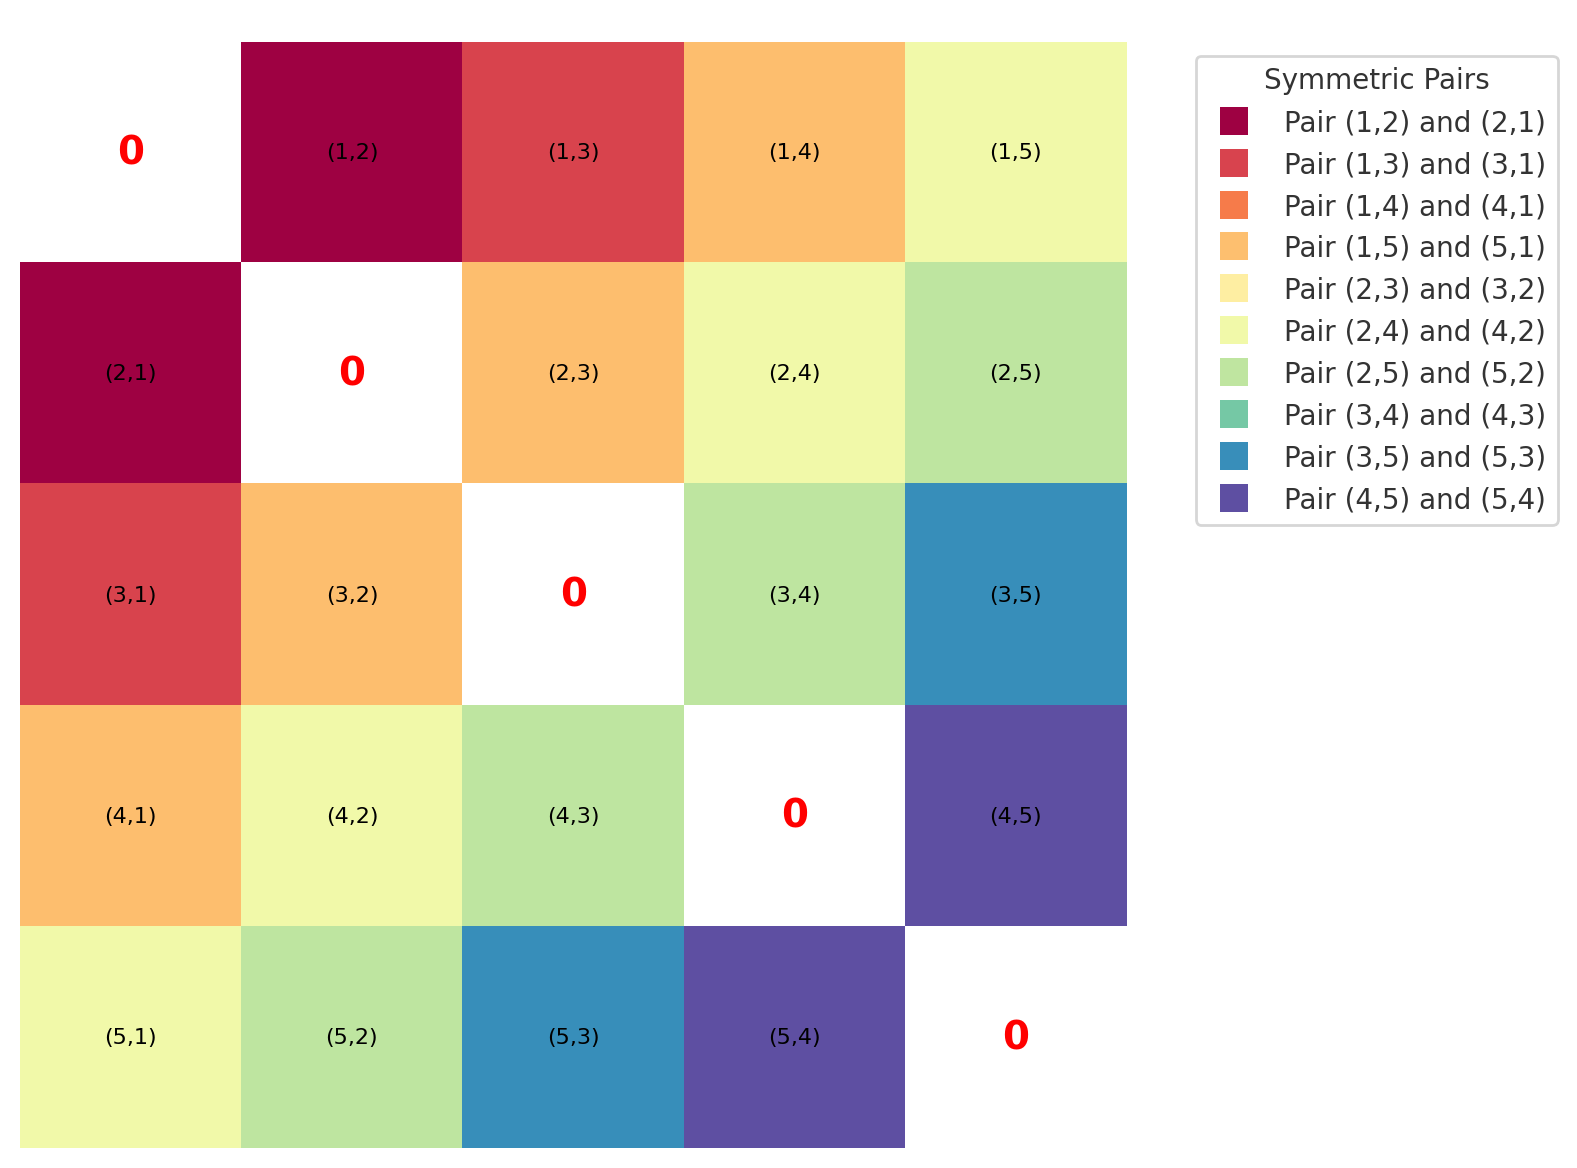
\includegraphics[width = 0.8\textwidth]{mtxvis.png}
    \caption{Visualization of $\sum_{i=1}^{n} \sum_{j=1}^{n} (a_ib_j-a_jb_i)$}
\end{figure}

With this image, we expand it until n; we can still cancel all elements symmetrical by the diagonal on by one. As the sum on the diagonal is 0, we conclude that 
$$\sum_{i=1}^{n} \sum_{j=1}^{n} (a_ib_j-a_jb_i)=0$$

Now consider the summation of squares. $(a_ib_j-a_jb_i)^2 = 0$ still holds for  $i=j$, but what about the symmetrical pairs $(i, j)$ and $(j, i)$?
We can figure it out by analysis by expanding the square of sum.
$$\sum_{i=1}^{n} \sum_{j=1}^{n}\left(a_{i}^{2} b_{j}^{2}-2 a_{i} a_{j} b_{i} b_{j}+a_{j}^{2} b_{i}^{2}\right)$$
By associative property of summation, we rearrange it as:
$$\sum_{i=1}^{n} \sum_{j=1}^{n}(a_i^2 b_j^2+a_j^2b_i^2) - 2\sum_{i=1}^{n} \sum_{j=1}^{n}a_ia_jb_ib_j$$
When $i \neq j$, each pair of $(i, j)$ and $(j, i)$. The sum of symmetric pair is
$$(a_i^2 b_j^2+a_j^2b_i^2 - 2a_ia_jb_ib_j) + (a_j^2 b_i^2+a_i^2b_j^2 - 2a_ia_jb_ib_j)$$
Rearrange it as:
$$2(a_i^2 b_j^2+a_j^2b_i^2) - 4(a_ia_jb_ib_j)$$
Still, as the sum of $(i, j)$ terms where $i=j$ is 0. We can ignore the diagonal. Hence, we have $n/2$ pairs
of $(a_i^2 b_j^2+a_j^2b_i^2) - 4(a_ia_jb_ib_j)$. This could be written as:
$$\frac{1}{2} \sum_{i=1}^{n} \sum_{j=1}^{n}2[(a_i^2 b_j^2+a_j^2b_i^2) - 4(a_ia_jb_ib_j)]$$
$$\sum_{i=1}^{n} \sum_{j=1}^{n}[(a_i^2 b_j^2+a_j^2b_i^2) - 2(a_ia_jb_ib_j)]$$
Notice that, $\sum_{i=1}^{n} \sum_{j=1}^{n}a_i^2 b_j^2 = \sum_{i=1}^{n} \sum_{j=1}^{n}a_j^2b_i^2$ due to the
diagonal symmetry of the summation as illustrated in the graph. We are adding the same term twice. 
Hence, we have:
$$2\sum_{i=1}^{n} \sum_{j=1}^{n}[a_i^2 b_j^2 - (a_ia_jb_ib_j)]$$
We can further simplify it by rule out the terms where $i=j$, as the summand is 0 in those cases.
We rewrite the sum as:
$$2\sum_{i=1}^{n-1} \sum_{j=2}^{n} [a_i^2 b_j^2 - (a_ia_jb_ib_j)]$$
or in single summation, we have:
$$2\sum_{i \neq j}[a_i^2 b_j^2 - (a_ia_jb_ib_j)] = 2\sum_{1 \leq i < j \leq n}[a_i^2 b_j^2 - (a_ia_jb_ib_j)] $$

For $\sum_{i=1}^{n} \sum_{j=1}^{n} (a_ib_j-a_jb_i)^n$, the symmetric property of summand still exists.
However we cannot prove it for now, as we need to use polynomial theorem to be introduced in Combinatorics.

%------------------------------------------------

\section{Sequence}
If everything so far is not a problem for you, congratulations, because you have known everything you need to know sequence. Sequence is an important concept that will be used throughout your journey of learning math. A Sequence
is defined as:
\begin{definition}[Sequence]\label{def_sequence}
    A sequence is a function \( f: \mathbb{N} \to \mathbb{R} \), where \(\mathbb{N}\) is the set of natural numbers and \(\mathbb{R}\) is the set of real numbers. The value \( f(n) \) 
    is the \( n \)-th term of the sequence, often denoted as \( a_n \). Therefore, a sequence can be represented as \( \{a_n\}_{n=1}^{\infty} \) for an infinite sequence or \( \{a_n\}_{n=1}^{N} \) for a finite sequence of length \( N \).
\end{definition} 

\subsection{Introduction}
Sequences could be either infinite or finite. A \textit{sequence} is defined to be a function \( S \) whose domain \( D \) is a nonempty interval of integers. \( S \) is an \textit{infinite sequence} if \( D \) has the form \( \{a..\} \). % Usually \( a \) is 1 or 0.

\( S \) is a \textit{finite sequence} if \( D \) has the form \( \{a..b\} \) where \( a \leq b \). When \( |D| = n \), we will say that \( S \) is an \( n\text{-sequence} \). We will take the domain of an \( n\text{-sequence} \) to be the set \( \{1..n\} \). % But \( a \) could be 0, and then \( D \) is \( \{0..(n - 1)\} \).

The (natural) ordering of the domain of a sequence \( S \) gives a natural ordering to the ordered pairs in the set \( S \). If \( S \) is a 5-sequence, then
\[ S = \{(1, S(1)), (2, S(2)), (3, S(3)), (4, S(4)), (5, S(5))\} \]

\begin{example}
    Suppose \( D = \{1..10\} \), and we define the function \( S \) on \( D \) by

\[ S(i) = \text{the smallest prime factor of the integer } (1 + i). \]

Then \( D \) is a finite interval of integers, and so \( S \) is the sequence denoted by

\[ S = (2, 3, 2, 5, 2, 7, 2, 3, 2, 11). \]
\end{example}

\begin{definition}[Sum of Sequence]
    If \( S = (S_1, S_2, S_3, \ldots, S_n) \) is a finite sequence of numbers, the corresponding \textit{series} is the sum of the entries in \( S \)
    is:

\[ S_1 + S_2 + S_3 + \ldots + S_n. \]
\end{definition}
\subsection{Special Sequences}
This section introduces common sequences as well as their properties.
\subsubsection{Algorithmic Sequence}
Algorithmic sequences are a fundamental concept in both computer science and mathematics, forming the backbone of algorithm design and analysis. These sequences are typically defined as an ordered set of steps or instructions, aimed at solving a specific problem or accomplishing a particular computation.
\begin{definition}[Arithmetic Sequence]
    An arithmetic sequence of the form
\[
a, a + d, a + 2d, \ldots, a + nd, \ldots
\]
where the initial term \( a \) and the common difference \( d \) are real numbers.
\end{definition}
Usually, the notation $a_n$ is used to express the nth term of a sequence (starting from 0). For the example in the 
definition, we have $a_0 = a$ and $a_n = a_0 + nd$. 
We also have:
$$a_1 = a_0 + d$$
$$a_2 = a_1 + d$$
$$\dots$$
$$a_n = a_0 + nd$$ 
for $n>=1$, $n\in \mathbb{Z}$:
$$a_n = a_{n-1} + d$$
These formula shows the linking between consecutive terms in an arithmetic sequence. We know that the sum
$s$ of the sequence is:
\begin{align*}
    S & =\ a_{0} \ +\ a_1\ \ +\ \dotsc \ +\ a\_n\\
    S & =\ a_{0} \ +\ a_{0} +d\ +\ \dotsc \ +\ a_{n-1} +d
    \end{align*}
The sum is expressed in infinite terms, and it is called \textbf{open form equation}. Accordingly, there are also \textbf{closed form
equations}.
\begin{definition}[Open Form]
    An \textit{open form} or \textit{non-closed form} expression, on the other hand, does not have a finite standard representation and often requires recursive or iterative methods for evaluation. It may involve summations, integrals, or other operations that are not easily simplified into a finite number of operations.
\end{definition}
\begin{definition}[Closed Form]
    A \textit{closed form} expression is a mathematical expression that can be evaluated in a finite number of standard operations. It typically involves constants, variables, and operations from algebra, calculus, and other areas of mathematics that can be computed in a finite number of steps.
    A closed form expression provides a direct way to compute the term of a sequence without the need for recursion.
\end{definition}

Is the open form good for calculating the sum of a sequence? Suppose now I want to know $S_{100}$ (The sum of the first 100th terms),
with the open form, I still have to calculate 99 terms using the definition of this sequence. So is there a way 
to make it possible that we get the sum in one step? Think about closed form. The closed form allows us to calculate
the sum directly. But is it possible to transform an open expression to closed form? If possible, how?

You may already notice that the open form has a property of infinity, and each step is somewhat related.
Isn't it a perfect problem to be solved by mathematical induction? We will leave this proof as a exercise, and here we provide another direct proof
by the symmetry of arithmetic sequence.
\begin{theorem}[Sum of Arithmetic Sequence]
    For  arithmetic sequence \( a_0, a_1, \ldots, a_{n-1} \), where each term can be expressed as \( a_i = a_0 + id \) and \( d \) is the common difference. The sum of the first nth terms is:
    \[ S = \frac{n}{2}[2a_0 + (n-1)d] \] or \[ S = \frac{n}{2}(a_0 + a_{n-1}) \] where \[ a_n = a_0 + nd \]
\end{theorem}
\begin{remark}
    We are trying to find the sum of the first n terms, and the first term is $a_0$, so the last term is
    $a_{n-1}$.
\end{remark}
\begin{proof}
    Consider an arithmetic sequence \( a_0, a_1, \ldots, a_n \), where each term can be expressed as \( a_i = a_0 + id \) and \( d \) is the common difference.
    \item Write the sum of the sequence in order:
\[
S = a_0 + (a_0 + d) + (a_0 + 2d) + \ldots + (a_0 + (n-1)d)
\]

\item Write the sum of the sequence in reverse order:
\[
S = (a_0 + (n-1)d) + (a_0 + (n-2)d) + \ldots + a_0
\]

\item Add these two equations together, every pair of terms within the brackets forms: \[ 2a_0 + (n-1)d \]

\item Since each term appears in a pair, there are \( n \) such pairs.

\item The resulting equation is \( 2S = n[2a_0 + (n-1)d] \).

\item Solving for \( S \) gives us \( S = \frac{n}{2}[2a_0 + (n-1)d] \) or \( S = \frac{n}{2}(a_0 + a_n) \), where \( a_n = a_0 + (n-1)d \).
\end{proof}


\subsubsection{Geometric Sequence}
Geometric sequence is the other important and common sequence that involved in problem-solving of computer
Science. 
A geometric sequence, also known as a geometric progression, is a sequence of numbers where each term after 
the first is found by multiplying the previous term by a fixed, non-zero number called the common ratio. 
Mathematically, a geometric sequence is defined as follows:
\begin{definition}[Geometric Sequence]
    Given the first term \( a_0 \) (also referred to as \( a_1 \) in some texts) and the common ratio \( r \), the \( n \)-th term of a geometric sequence \( a_n \) can be expressed as:
\[
a_n = a_0 \cdot r^n \quad \text{for } n \geq 0
\]
where \( n \) is a non-negative integer representing the position of the term in the sequence.
\end{definition}    

The common ratio \( r \) can be any real number. If \( |r| < 1 \), the terms of the sequence 
will get progressively smaller and approach zero. If \( |r| > 1 \), the terms will grow progressively 
larger. If \( r = 1 \), the sequence is constant, and if \( r = -1 \), the sequence will alternate 
between two values.

We can deduce the sum of a specific geometric sequence by direct proof.
\begin{theorem}[Sum of Geometric Sequence]
    
\end{theorem}

\begin{proof}
    Consider a geometric sequence with the first term \( a_0 \) and the common ratio \( r \) where \( r \neq 1 \). The sequence is given by:
\[ a_0, a_0r, a_0r^2, \ldots, a_0r^{n-1} \]

The sum of the first \( n \) terms of the sequence, denoted by \( S_n \), is:
\[ S_n = a_0 + a_0r + a_0r^2 + \ldots + a_0r^{n-1} \]

To find a formula for \( S_n \), multiply the entire sequence by \( r \):
\[ rS_n = a_0r + a_0r^2 + a_0r^3 + \ldots + a_0r^n \]

Subtract the original sum \( S_n \) from this new sum \( rS_n \) to get a telescoping series:
\[ rS_n - S_n = a_0r^n - a_0 \]

Solving for \( S_n \) gives us:
\[ S_n = \frac{a_0(1 - r^n)}{1 - r} = \]

This is the sum formula for the first \( n \) terms of a geometric sequence when \( r \neq 1 \). If \( r = 1 \), the sequence is constant, and the sum of the first \( n \) terms is simply \( n \) times the first term \( a_0 \).
\end{proof}
%----------------------------------------------------------------------
\subsubsection{characteristic Sequence}
\begin{definition}[Characteristic Sequence]
    Suppose that \( U \) is some given \( n \)-set whose elements have been \textit{indexed} (listed in a certain order) so that \( U = \{x_1, x_2, \ldots, x_n\} \). If \( A \) is a subset of \( U \), the \textit{characteristic sequence} of \( A \) is the function whose domain is \( \{1..n\} \) defined by

\[
X^A_i = X^A(i) = 
\begin{cases} 
1 & \text{if } x_i \in A \\
0 & \text{if } x_i \notin A 
\end{cases}
\]
\end{definition}

\begin{example}
    If \( U \) is the set of the first 10 odd positive integers, \( A \) is the subset of primes in \( U \), and \( B \) is the set of multiples of 3 in \( U \), then
    
    \[
    \begin{aligned}
    &U = \{1, 3, 5, 7, 9, 11, 13, 15, 17, 19\} &&// x_i = 2i - 1. \\
    &A = \{3, 5, 7, 11, 13, 17, 19\} \\
    &B = \{3, 9, 15\} \\
    &X^A = (0, 1, 1, 1, 0, 1, 1, 0, 1, 1) \\
    &X^B = (0, 1, 0, 0, 1, 0, 0, 1, 0, 0).
    \end{aligned}
    \]
    \end{example}

    Characteristic sequences may be used as an implementation model for subsets of any given indexed set \( U \). The set operations may be done on these sequences:
    \[
    X^{A \cap B}_i = X^A_i \times X^B_i;
    \]
    \[
    X^{A \cup B}_i = X^A_i + X^B_i - X^A_i \times X^B_i;
    \]
    \[
    X^{A \setminus B}_i = X^A_i - X^A_i \times X^B_i.
    \]
    
    If \( A \subseteq B \) then
    \[
    X^A_i \leq X^B_i \quad \text{for each index } i,
    \]
    and
    \[
    |A| = \sum_{i=1}^{n} X^A_i.
    \]

%----------------------------------------------------------------------
\subsection{Exercises}
\begin{exercise}
    Find the sum of arithmetic sequence using mathematical induction. Try \textbf{NOT} use the conclusion in this section.
\end{exercise}
Hint: Consider the sum of the first nth positive integer. Try to make assumption by taking it as an arithmetic sequence.
\begin{proof}
    Let \( S(n) \) denote the sum of the first \( n \) terms of an arithmetic sequence with the first term \( a_0 \) and common difference \( d \).
    \begin{itemize}
        \item \textbf{Base Case (\( n = 1 \))}: The sum of the sequence with only the first term is the first term itself, \( S(1) = a_0 \).
        \item \textbf{Inductive Step}: Assume that the sum of the first \( k \) terms \( S(k) \) is given by a certain formula. We want to show that the sum of the first \( k+1 \) terms \( S(k+1) \) can be expressed using the same formula.
        \end{itemize}
        
        For the base case, we can easily see that:
        \[
        S(1) = a_0
        \]
        As $\sum_{1}^{n}i = \frac{n(n+1)}{2}$, which could be taken as an arithmetic sequence with $a_0=1$ and
        $a_n=n$.
        By this, assume that the sum of the first \( k \) terms is:
        \[
        S(k) = \frac{k}{2} [a_0 + a_n]
        \]
        equivalent to
        \[
        S(k) = \frac{k}{2} [2a_0 + (k-1)d]
        \]
        
        To prove the inductive step for \( S(k+1) \), consider:
        \[
        S(k+1) = S(k) + a_0 + kd
        \]
        
        Substituting the inductive hypothesis into the above equation yields:
        \[
        S(k+1) = \frac{k}{2} [2a_0 + (k-1)d] + a_0 + kd
        \]
        
        After simplifying, we aim to show that:
        \[
        S(k+1) = \frac{k+1}{2} [2a_0 + kd]
        \]
        
        This will complete the proof if we can establish that the simplified version of \( S(k+1) \) matches the form of the inductive hypothesis.
\end{proof}
\begin{exercise}
    Prove the sum of geometric sequence  is \( S_n = \frac{a_0(1 - r^n)}{1 - r} = \) using mathematical induction.
\end{exercise}
\begin{proof}
    We want to prove that the sum of the first \( n \) terms of a geometric sequence \( S_n \) with the first term \( a \) and common ratio \( r \) (where \( r \neq 1 \)) is given by:

\[ S_n = \frac{a(1 - r^n)}{1 - r} \]

\textbf{Base Case (n=1):}

The sum of the first term is simply the term itself:

\[ S_1 = a \]

which agrees with the formula.

\textbf{Inductive Step:}

Assume the formula holds for \( n = k \), that is,

\[ S_k = \frac{a(1 - r^k)}{1 - r} \]

We need to prove that it also holds for \( n = k+1 \):

\[ S_{k+1} = \frac{a(1 - r^{k+1})}{1 - r} \]

Starting with the inductive hypothesis for \( S_k \) and adding the \( (k+1) \)-th term \( ar^k \) to both sides, we have:

\[ S_k + ar^k = \frac{a(1 - r^k)}{1 - r} + ar^k \]

Simplifying, we obtain:

\[ S_{k+1} = S_k + ar^k = \frac{a - ar^{k+1}}{1 - r} \]

which is the same as the formula for \( S_{k+1} \), thus completing the proof.
\end{proof}
\begin{exercise}
    Given a sequence \( \{a_n\} \) and a series \( S_n = an^2 + bn + c (a \neq 0) \).

\begin{enumerate}
    \item Find the general term \( a_n \);
    \item Is the sequence \( \{a_n\} \) an arithmetic sequence?
\end{enumerate}
\end{exercise}
Hint: How can we get the value of a term from the sum of a sequence?
\textbf{Solution:}

\begin{enumerate}
    \item For \( n \geq 2 \), \( a_n = S_n - S_{n-1} = (an^2 + bn + c) - [a(n-1)^2 + b(n-1) + c] \) \\
    \( = (b+a) + (n-1) \cdot 2a \),
    
    Therefore, for \( n=1 \), \( a_1 = (b+a) + (1-1) \cdot 2a = b + a + c - S_1 \), \\
    and the general term is
    \[
    a_n = 
    \begin{cases}
        a + b + c & (n=1) \\
        (b+a) + (n-1) \cdot 2a & (n \geq 2)
    \end{cases}
    \]

    \item Since \( c = 0 \), \( a_n \) can be simplified to \( a_n = a + b \), which is constant and equals \( 2a \) when \( n \geq 2 \). This implies \( \{a_n\} \) is an arithmetic sequence with common difference \( 2a \), provided \( a, b \) are constants and \( a \neq 0 \).
    
    Note: From \( S_n \) we can deduce \( a_n = S_n - S_{n-1} \) when \( n \geq 2 \). Since \( a_1 = S_1 \), the sequence \( a_n = S_n - S_{n-1} \) (for \( n \geq 2 \)) and \( a_1 \) is the first term. The sequence \( \{a_n\} \) is an arithmetic sequence.
    
    Therefore, the general term \( a_n \) can be expressed as:
    \[
    a_n = 
    \begin{cases}
        S_1 & (n=1) \\
        S_n - S_{n-1} & (n \geq 2)
    \end{cases}
    \]
    
    Given the series \( \{a_n\} \) with \( S_n = an^2 + bm + c (a \neq 0) \), the sequence \( \{a_n\} \) is an arithmetic sequence with common difference \( 2a \) when \( c = 0 \).
\end{enumerate}

\begin{exercise}
    Given constants $a$, $b$, $c$, consider the sum $S_n = 1^2 + 2^2 + 3^2 + \ldots + n(n+1)^2 = \frac{n(n+1)}{12}(an^2 + bn + c)$, where $an^2 + bn + c \neq 0$.
\end{exercise}
\begin{proof}
    For $n=1$, we have $\frac{1}{6}(a+b+c)$, thus $a_1 = 4 = \frac{1}{6}(a+b+c)$.
For $n=2$, we have $\frac{22}{2} = 11 = \frac{1}{2}(4a+b+c)$, thus $a_2 = 22 = 9a + 3b + c$.
For $n=3$, $a_3 = 70 = 9a + 3b + c$.\\

From these equations, we find that:
\begin{align*}
    a + b + c &= 24 \\
    4a + b + c &= 44 \\
    9a + 3b + c &= 70
\end{align*}

Solving the system, we get $a=3$, $b=11$, $c=10$.
For \(n = 1, 2, 3\), the sum can be expressed as:
\[
1 \cdot 2^2 + 2 \cdot 3^2 + \ldots + n(n+1)^2 = \frac{n(n+1)}{12}(3n^2 + 11n + 10),
\]
thus, \(S_n = 1 \cdot 2^2 + 2 \cdot 3^2 + \ldots + n(n+1)^2\).

For a general term \(k\), \(S_k = \frac{k(k+1)}{12}(3k^2 + 11k + 10)\). Therefore,
\[
S_{k+1} = S_k + (k+1)(k+2)^2
\]
\[
= \frac{k(k+1)}{12}(3k^2 + 11k + 10) + (k+1)(k+2)^2
\]
\[
= \frac{k(k+1)}{12}((k+2)(3k+5) + (k+1)(k+2)^2)
\]
\[
= \frac{(k+1)(k+2)}{12}(3k^2 + 5k + 12k + 24)
\]
\[
= \frac{(k+1)(k+2)}{12}(3(k+1)^2 + 11(k+1) + 10).
\]

Hence, by induction, we can show that for \(n = k+1\) the sum is valid.

Finally, with \(a = 3\), \(b = 11\), \(c = 10\), we confirm that the given sequence is indeed a second-order arithmetic sequence.
\end{proof}

\begin{exercise}
    Evaluate:
    \begin{enumerate}
        \item $S = \sum_{1}^{n} \frac{N}{2^n}$
        \\
        \item $S = \sum_{1}^{n} \frac{3n-2}{5^{n-1}}$  
    \end{enumerate}
\end{exercise}

\textbf{Solution:}

(1) Given the series \( S_n = \frac{1}{2} + \frac{2}{4} + \frac{3}{8} + \cdots + \frac{n}{2^n} \), we can write:

\[
S_n - \frac{1}{2}S_n = \frac{1}{2} + \frac{1}{4} + \frac{1}{8} + \cdots + \frac{1}{2^n} - \frac{n}{2^{n+1}}
\]

This simplifies to:

\[
\frac{1}{2}S_n = \frac{1}{2} \left(1 - \left(\frac{1}{2}\right)^n\right) = \frac{1}{2} - \frac{1}{2^{n+1}} = \frac{1}{2} - \frac{n}{2^{n+1}} + \frac{n}{2^{n+1}}
\]

Hence, the series sum is:

\[
S_n = 2 - \frac{1}{2^{n-1}} - \frac{n}{2^n} = 2 - \frac{n+2}{2^n}
\]

(2) Considering the series \( S_n = 1 + \frac{4}{5} + \frac{7}{25} + \cdots + \frac{3n-2}{5^{n-1}} \), we proceed similarly:

\[
\left(1 - \frac{1}{5}\right)S_n = 1 + \frac{3}{5} + \frac{3}{25} + \cdots + \frac{3}{5^{n-1}} - \frac{3n-2}{5^n}
\]

The terms form a geometric series, so we get:

\[
S_n = 1 + \frac{3}{5} \left(1 + \frac{1}{5} + \frac{1}{25} + \cdots + \frac{1}{5^{n-2}}\right) - \frac{3n-2}{5^n}
\]

Applying the formula for the sum of a geometric series, we find:

\[
S_n = 1 + \frac{3}{5} \left(\frac{1 - \left(\frac{1}{5}\right)^{n-1}}{1 - \frac{1}{5}}\right) - \frac{3n-2}{5^n}
\]

Simplifying, we obtain:

\[
S_n = 1 + \frac{3}{5} \left(\frac{5^n - 5}{4 \cdot 5^{n-1}}\right) - \frac{3n-2}{5^n}
\]

Further simplification gives us:

\[
S_n = \frac{35}{16} - \frac{12n+7}{16 \cdot 5^{n-1}}
\]
%------------------------------------------------